%%
%% Copyright (c) 2019 Weitian LI <liweitianux@sjtu.edu.cn>
%% Creative Commons BY 4.0
%%

\documentclass{beamer}

\usetheme{metropolis}
\metroset{progressbar=foot}

\setbeamertemplate{section in toc}[sections numbered]
% Numbered sections in section page
% Credit: https://github.com/matze/mtheme/issues/271#issuecomment-292799444
\makeatletter
\setbeamertemplate{section page}{
  \centering
  \begin{minipage}{25em}
    \raggedright
    \usebeamercolor[fg]{section title}
    \usebeamerfont{section title}
    \thesection.~\insertsectionhead\\[-1ex]
    \usebeamertemplate*{progress bar in section page}
    \par
    \ifx\insertsubsectionhead\@empty\else%
      \usebeamercolor[fg]{subsection title}%
      \usebeamerfont{subsection title}%
      \thesection.\thesubsection.~\insertsubsectionhead
    \fi
  \end{minipage}
  \par
  \vspace{\baselineskip}
}
\makeatother

\setbeamertemplate{frametitle continuation}{(\insertcontinuationcount)}
\setbeamertemplate{bibliography item}{\insertbiblabel}

\setbeamertemplate{itemize items}[circle]
\setbeamertemplate{itemize subitem}[triangle]
% Suppress itemize indentation
% Credit: https://tex.stackexchange.com/a/450317
\settowidth{\leftmargini}{\usebeamertemplate{itemize item}}
\addtolength{\leftmargini}{\labelsep}
\settowidth{\leftmarginii}{\usebeamertemplate{itemize subitem}}
\addtolength{\leftmarginii}{\labelsep}

% Solarized theme
% Credit: https://ethanschoonover.com/solarized/
\definecolor{SolBase02}{HTML}{073642}
\definecolor{SolBase3}{HTML}{fdf6e3}
\definecolor{SolOrange}{HTML}{cb4b16}
\definecolor{SolGreen}{HTML}{859900}
%
\setbeamercolor{normal text}{fg=SolBase02, bg=SolBase3}
\setbeamercolor{alerted text}{fg=SolOrange}
\setbeamercolor{example text}{fg=SolGreen}

\setsansfont{Fira Sans Light}[
  BoldFont={Fira Sans Medium}
]
\setmonofont{Fira Code Light}[
  BoldFont={Fira Code Medium}
]

\usepackage{bm}
\usepackage{newtxsf}
\newcommand{\R}[1]{\text{#1}}  % text math alphabets
\newcommand{\Ce}{\R{e}}  % constant e
\newcommand{\Ci}{\R{i}}  % constant i
\newcommand{\Cpi}{\piup}  % upright 'pi', provided by 'newtxsf' package
\newcommand{\B}[1]{\bm{\mathsf{#1}}}  % single-letter bold math
\newcommand{\D}[1]{\R{d}#1}
\newcommand{\diff}[2]{\frac{\D{#1}}{\D{#2}}}
\newcommand{\pdiff}[2]{\frac{\partial #1}{\partial #2}}

\usepackage{xeCJK}
\setCJKsansfont{Source Han Sans SC Light}[
  BoldFont={Source Han Sans SC Medium}
]

\usepackage{hyperref}
\hypersetup{
  pdfstartview={Fit}
}

\usepackage{appendixnumberbeamer}
\usepackage{booktabs}
\usepackage{csquotes}

\usepackage{caption}
\captionsetup{%
  figurename={图},
  format=plain,
  labelformat=simple,
  labelsep=period,
  justification=centering,
  textfont={footnotesize},
  labelfont={footnotesize},
}

\usepackage{keyval}
\usepackage{etoolbox}

\makeatletter
% Set the keys (arguments) for including a figure
\newlength{\myfigure@width}
\newlength{\myfigure@height}
\newtoggle{myfigure@vertcap}
\define@key{myfigure}{width}{\setlength\myfigure@width{#1}}
\define@key{myfigure}{height}{\setlength\myfigure@height{#1}}
\define@key{myfigure}{vertcap}[true]{\toggletrue{myfigure@vertcap}}
%
% Custom command to include a figure with a horizontal/vertical caption
\NewDocumentCommand{\myfigure}{m m m}{
  \setkeys{myfigure}{width=0pt, height=0pt, #1}
  %
  % Get the size that a figure is being rendered
  % Credit: https://tex.stackexchange.com/a/3664
  \newsavebox{\myfigure@box}
  \ifdimequal{\myfigure@height}{0pt}{
    \savebox{\myfigure@box}{%
      \includegraphics[width=\myfigure@width]{#2}}
  }{%
    \savebox{\myfigure@box}{%
      \includegraphics[height=\myfigure@height]{#2}}
  }
  \settowidth{\myfigure@width}{\usebox{\myfigure@box}}
  \settoheight{\myfigure@height}{\usebox{\myfigure@box}}
  %
  \begin{figure}[!h]
    \centering
    \usebox{\myfigure@box}
    \iftoggle{myfigure@vertcap}{%
      \hspace{-0.5em}%
      % Credit: https://tex.stackexchange.com/a/44433
      \rotatebox{90}{%
        \begin{minipage}{\myfigure@height}
          \caption{#3}
        \end{minipage}
      }
    }{%
      \caption{#3}
    }
  \end{figure}
  % Credit: https://tex.stackexchange.com/a/18174
  \global\let\myfigure@box\relax
}
%
\makeatother

\usepackage{xparse}
% Credit: https://tex.stackexchange.com/a/376366
\ExplSyntaxOn
\NewDocumentCommand{\cspace}{O{1em}}{%
  \tl_map_inline:nn {空} { \makebox[#1]{\phantom{##1}} }
}
\ExplSyntaxOff

\usepackage{siunitx}
% siunitx settings and new units
\sisetup{
  range-phrase=\text{--},
  range-units=single,
  product-units=repeat,
  list-separator={, },
  list-final-separator={, and },
  separate-uncertainty=true,
  detect-all,  % detecting fonts
}
%
\DeclareSIUnit\arcsec{arcsec}
\DeclareSIUnit\arcmin{arcmin}
\DeclareSIUnit\cMpc{cMpc}  % comoving Mpc
\DeclareSIUnit\cGpc{cGpc}  % comoving Gpc
\DeclareSIUnit\deg{deg}
\DeclareSIUnit\dyne{dyn}
\DeclareSIUnit\erg{erg}
\DeclareSIUnit\esu{esu}
\DeclareSIUnit\franklin{Fr}
\DeclareSIUnit\gauss{G}
\DeclareSIUnit\hubble{\ensuremath{\mathit{h}}}
\DeclareSIUnit\jansky{Jy}
\DeclareSIUnit\lightyear{ly}
\DeclareSIUnit\parsec{pc}
\DeclareSIUnit\rayleigh{Rayleigh}
\DeclareSIUnit\solarmass{\ensuremath{\mathrm{M}_{\odot}}}
\DeclareSIUnit\statcoulomb{statC}
\DeclareSIUnit\year{yr}
%
\DeclareSIUnit\kpc{\kilo\parsec}
\DeclareSIUnit\mJy{\milli\jansky}
\DeclareSIUnit\mK{\milli\kelvin}
\DeclareSIUnit\Gpc{\giga\parsec}
\DeclareSIUnit\Gyr{\giga\year}
\DeclareSIUnit\Mpc{\mega\parsec}
\DeclareSIUnit\Myr{\mega\year}
\DeclareSIUnit\uG{\micro\gauss}

\usepackage{journalabbrv}

\usepackage[%
  backend=biber,
  style=numeric,
  sorting=none,
  autocite=superscript,
]{biblatex}
%
% Credit: https://tex.stackexchange.com/a/60923
\DeclareCiteCommand{\cite}[\mkbibsuperscript]%
  {\iffieldundef{prenote}
     {}
     {\BibliographyWarning{Ignoring prenote argument}}%
   \iffieldundef{postnote}
     {}
     {\BibliographyWarning{Ignoring postnote argument}}}
  {\usebibmacro{citeindex}%
   \bibopenbracket\usebibmacro{cite}\bibclosebracket}
  {\supercitedelim}
  {}
\newcommand{\citeay}[1]{\citeauthor{#1} \citeyear{#1} \parencite{#1}}

\AtBeginBibliography{
  \linespread{1.0}
  \footnotesize
}
\addbibresource{../references.bib}

\graphicspath{
  {./}
  {figures/}
  {../figures/}
  {../figures/self/}
  {../sjtuthesis/}
}

% Change 'emph' style to bold face
\let\emph\relax  % there's no \RedeclareTextFontCommand
\DeclareTextFontCommand{\emph}{\boldmath\bfseries}

\newcommand{\email}[1]{\href{mailto:#1}{\texttt{#1}}}
\newcommand{\doi}[1]{\href{https://doi.org/#1}{\textsc{doi}:#1}}
\newcommand{\ads}[1]{\href{http://adsabs.harvard.edu/abs/#1}{\textsc{ads}:#1}}
\newcommand{\arxiv}[1]{\href{https://arixv.org/abs/#1}{\textsc{arXiv}:#1}}


%=====================================================================

\title[探测宇宙再电离时期]{%
  射电晕对宇宙再电离探测的影响和\texorpdfstring{\\}{}%
  基于深度学习的再电离信号分离新算法%
}
\author[李维天]{李维天 <\email{liweitianux@sjtu.edu.cn}>}
\institute{%
  物理与天文学院\\%
  上海交通大学%
}
\date{\small 2019 年 6 月 ?? 日}  % TODO
\subject{博士学位论文答辩}
\titlegraphic{%
  
\includegraphics[height=0.75cm]{sjtubadge}%
  \hspace{2mm}%
  
\includegraphics[height=0.75cm]{sjtulogo}%
}


%=====================================================================

\begin{document}

\maketitle

\begin{frame}{目\cspace{}录}
  \tableofcontents[hideallsubsections]
\end{frame}


%=====================================================================
\section{绪论}

%............
\begin{frame}{研究背景}
  \begin{itemize}
    \item 我们对宇宙的\alert{中期历史}仍然知之甚少,可细分为 \cite{koopmans2015}:\\
      无知时期 ($z \sim \numrange{200}{1100}$)、
      黑暗时期 ($z \sim \numrange{30}{200}$)、\\
      黎明时期 ($z \sim \numrange{15}{30}$)、
      \alert{再电离时期 (EoR; $z \sim \numrange{6}{15}$)}.
    \item \alert{中性氢 21\,cm 谱线} ($\sim$\,\SI{1420}{\MHz})
      是探测 EoR 以及更早的黑暗时期的最直接而有效的探针.
    \item EoR 信号将出现在 $\sim$\,\SIrange{90}{200}{\MHz} 的低频射电波段.
  \end{itemize}

  \vspace{-1ex}
  \myfigure{%
    width=0.85\textwidth,
    vertcap,
  }{universe-history}{宇宙的演化历史\\(来源: BICEP2/CERN/NASA)}
\end{frame}

%............
\begin{frame}
  \begin{itemize}
    \item EoR 信号非常微弱,亮温度仅约几 mK 至十几 mK.
    \item 前景干扰非常强烈,多种前景干扰成分.
    \item 仪器效应复杂、观测干扰显著、数据处理困难、等等.
    \item 亟待深入理解前景干扰,构建准确的前景模型,
      研发有效的前景处理和 EoR 信号分离算法,
      才能保障 EoR 探测实验的成功.
  \end{itemize}

  \vspace{-1ex}
  \myfigure{%
    width=0.8\textwidth,
    vertcap,
  }{eor-foregrounds}{主要前景成分示意图\\(\citeay{zaroubi2013})}
\end{frame}

%............
\begin{frame}{研究内容}
  \begin{alertblock}{1. 改进射电晕的建模以及评估其对 EoR 探测的影响}
    \begin{itemize}
      \item 星系团射电晕是一类典型的河外射电展源:\\
        尺度较大(若干角分)、形态相对复杂、
        数目较多(SKA 将发现约 2500 个 \cite{cassano2015}),
        可能对 EoR 信号的探测产生显著干扰.
      \item 相比银河系以及河外点源等前景成分,对射电晕的研究明显不足而且比较粗糙.
      \item 基于\alert{湍流再加速模型},模型星系团的形成与演化过程,
        显著改进射电晕的低频射电天图的模拟.
      \item 采用 \alert{SKA1-Low 阵列布局},整合逼真的干涉阵列仪器效应.
      \item 利用一维和二维功率谱,量化射电晕对 EoR 信号的干扰情况,
        指导 EoR 实验的数据处理以及 EoR 信号分离算法的研发.
    \end{itemize}
  \end{alertblock}
\end{frame}

%............
\begin{frame}{研究内容}
  \begin{alertblock}{2. 基于深度学习研发 EoR 信号分离新算法}
    \begin{itemize}
      \item 传统的前景处理方法依赖于:前景辐射的频谱必须非常光滑.
      \item 干涉阵列的波束存在频率依赖效应,导致前景辐射的频谱出现小尺度涨落,
        光滑性受到损坏.
      \item 波束形状非常复杂,难以为现有方法打造一个实际可用的波束模型.
      \item 深度学习方法能从数据中学习知识并自适应地优化自身模型.
      \item 基于深度学习方法研发 EoR 信号分离新算法更加可行、更具有吸收力.
    \end{itemize}
  \end{alertblock}
\end{frame}


%=====================================================================
\section{射电天文学基础}

%............
\begin{frame}{射电天文学}
  \alert{射电天文学}:
  在射电波段对天体和宇宙开展研究的天文学分支.
  \alert{射电窗口}的频率范围 $\sim$ \SI{10}{\MHz} -- \SI{1000}{\GHz}.

  \begin{figure}
    \centering
    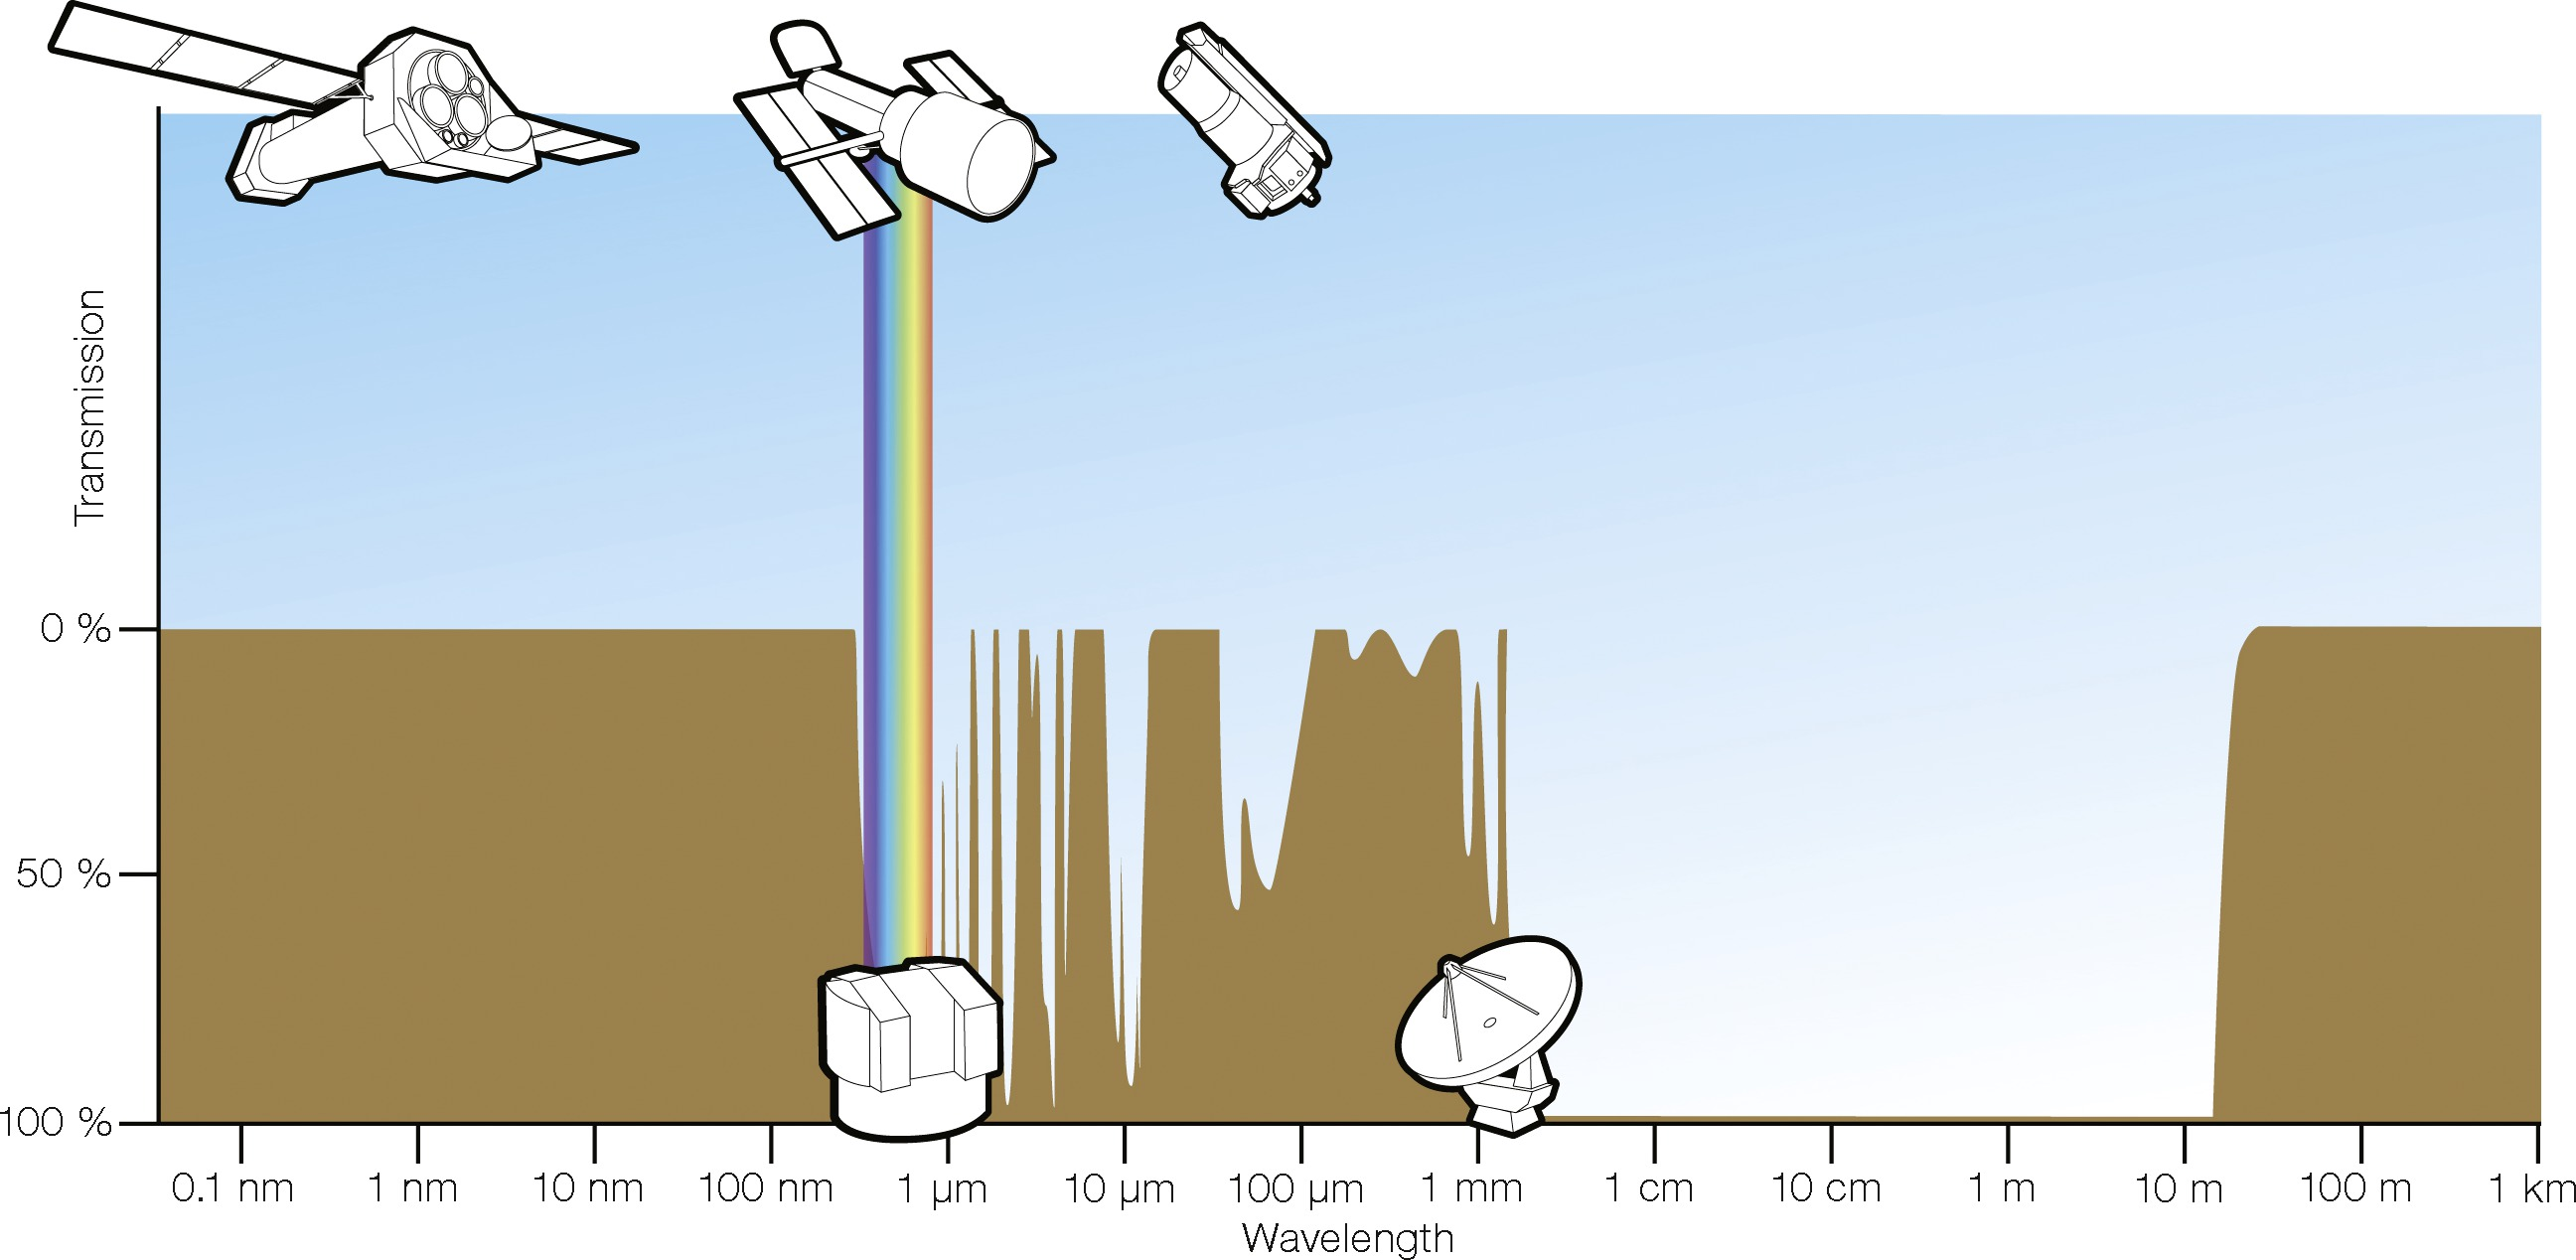
\includegraphics[width=\textwidth]{atmospheric-em-transmittance}
    \caption{大气层的电磁辐射透射率 (来源: \citeay{condon2016})}
  \end{figure}
\end{frame}

%............
\begin{frame}{比强度和流量密度}
  \begin{columns}
    \column{0.6\textwidth}
      \begin{alertblock}{比强度 (specific intensity)}
        \smallskip
        单位频率间隔内、沿着辐射传播方向上单位立体角穿过垂直于传播方向的单位面积
        的辐射功率,即:
        \begin{equation}
          I_{\nu} \equiv
            \frac{\D{P_{\nu}}}{(\cos\theta\,\D{\sigma})
              \,\D{\nu} \,\D{\Omega}} \,,
        \end{equation}
        亦被称为\emph{谱亮度},或简称\emph{强度}或\emph{亮度}.
      \end{alertblock}

      \begin{alertblock}{流量密度 (flux density)}
        \smallskip
        \begin{equation}
          S_{\nu} \equiv
            \int_{\R{source}} I_{\nu}(\theta,\phi) \cos\theta \,\D{\Omega} ,
        \end{equation}
        单位为 \si{\jansky},
        $\SI{1}{\jansky} = \SI{e-26}{\watt\per\square\meter\per\hertz}$.
      \end{alertblock}

    \column{0.4\textwidth}
      \begin{figure}
        \centering
        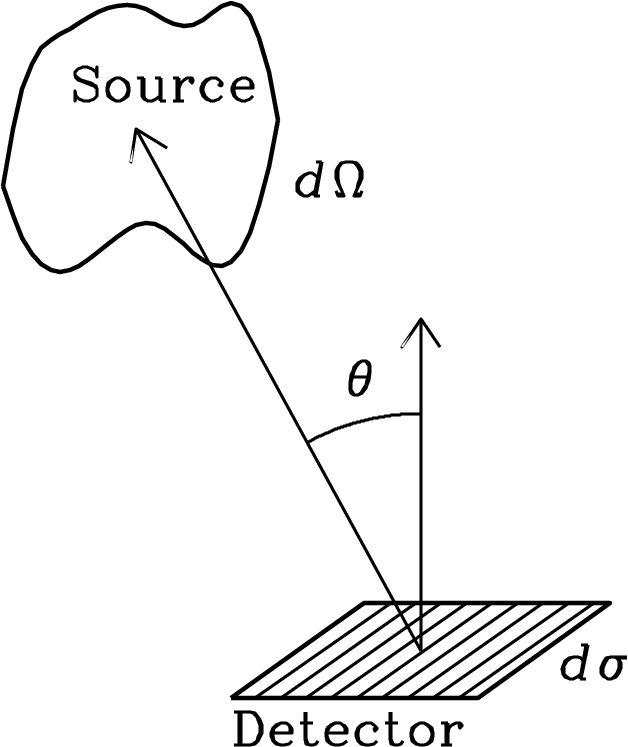
\includegraphics[width=0.9\columnwidth]{specific-intensity}
        \caption{比强度 $I_{\nu}$ 测量示意图 (\citeay{condon2016})}
      \end{figure}
  \end{columns}
\end{frame}

%............
\begin{frame}{亮温度}
  \begin{itemize}
    \item \alert{黑体辐射}的频谱 $B_{\nu}(\nu, T)$ 只取决于其温度 $T$,
      由 \alert{Planck 定律}给出:
      \begin{equation}
        B_{\nu}(\nu, T) =
          \frac{2 h_p \nu^3}{c^2} \left[ \exp\left(
            \frac{h_p \nu}{k_B T} \right) - 1 \right]^{-1} .
      \end{equation}
    \item 在射电波段有 $h_p \nu \ll k_B T$,于是有 \alert{Rayleigh--Jeans 近似}:
      \begin{equation}
        B_{\nu}(\nu, T) \approx \frac{2 \nu^2 k_B T}{c^2} .
      \end{equation}
      黑体的亮度 $B_{\nu}$ 与其温度 $T$ 严格成正比.
    \item 一个辐射源的亮度 $I_{\nu}$ 可以很方便与使用\alert{亮温度}来描述:
      \begin{equation}
        T_b(\nu) \equiv \frac{I_{\nu} c^2}{2 k_B \nu^2} .
      \end{equation}
  \end{itemize}
\end{frame}


%=====================================================================
\section{再电离时期的探测}

%............
\begin{frame}{中性氢 21\texorpdfstring{\,}{ }cm 谱线}
  \begin{columns}
    \column{0.55\textwidth}
    \begin{itemize}
      \item 质子和电子均有 1/2 自旋.
      \item 两个自旋的相互作用使氢原子的基态发生\alert{超精细分裂}.
      \item 当电子的自旋发生翻转时,会产生/吸收频率约为 \SI{1420}{\MHz} 的光子,
        波长约为 21\,cm,因此被称为 \alert{21\,cm 谱线}.
    \end{itemize}

    \column{0.45\textwidth}
    \begin{figure}
      \centering
      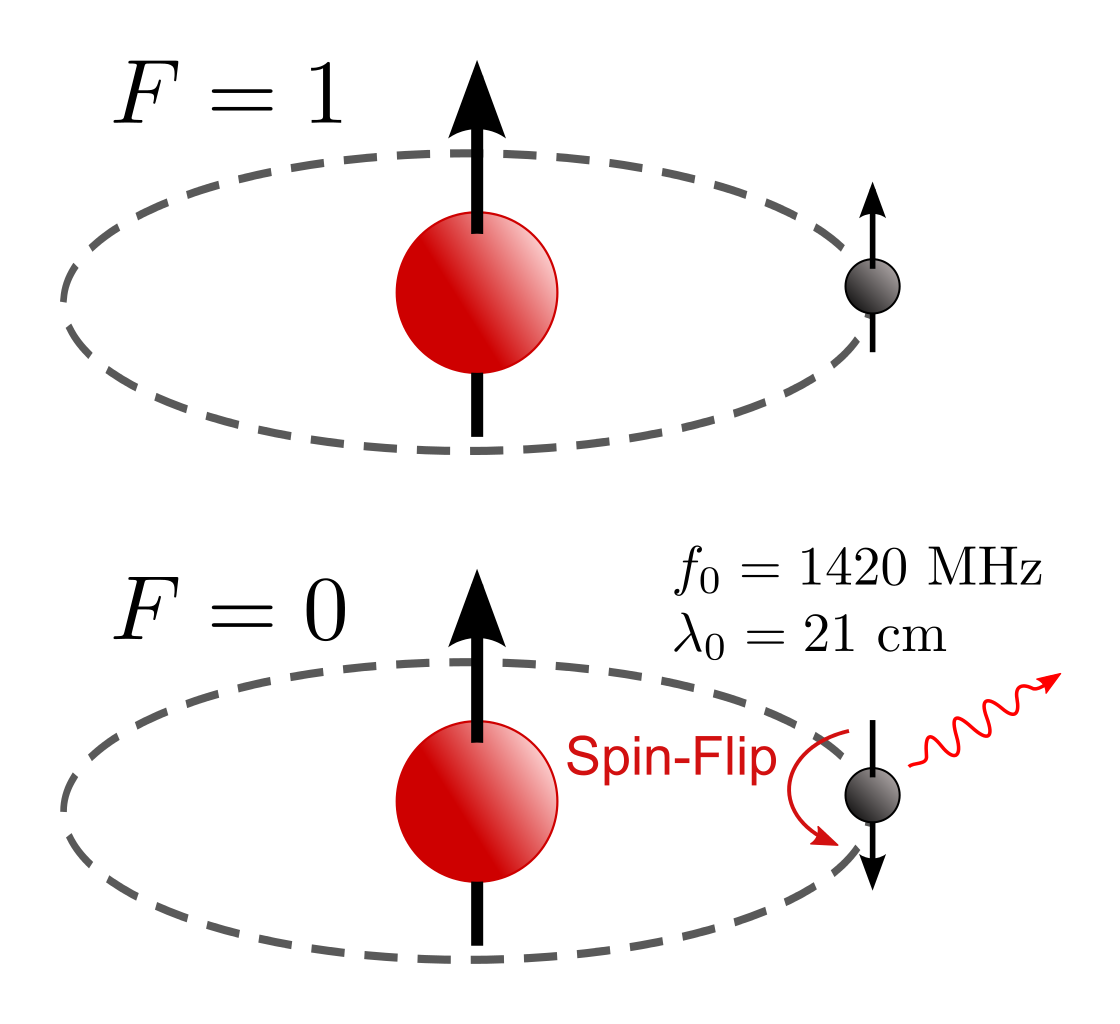
\includegraphics[width=\columnwidth]{hydrogen-spinflip}
      \caption{氢原子的自旋翻转跃迁\\(来源: Tiltec, Wikipedia)}
    \end{figure}
  \end{columns}
\end{frame}

%............
\begin{frame}{EoR 信号}
  \begin{figure}
    \centering
    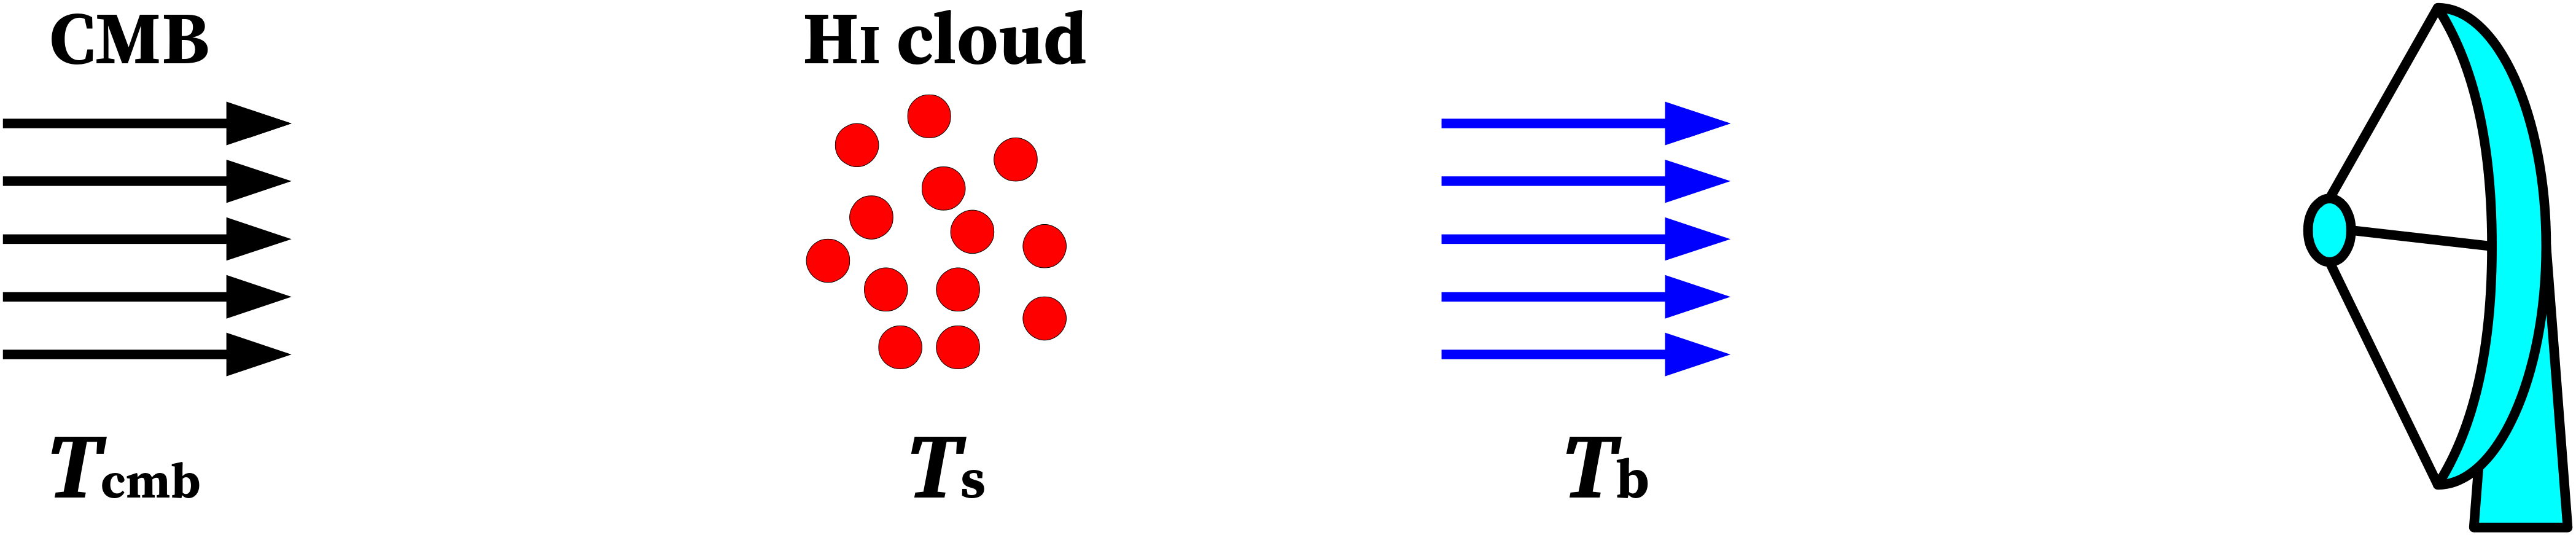
\includegraphics[width=\textwidth]{21cm-radiative-transfer}
    \caption{CMB 辐射穿过中性氢云的辐射转移示意图 (\citeay{zaroubi2013})}
  \end{figure}

  待探测的 \alert{EoR 信号}为中性氢云的辐射相对于 CMB 辐射的\alert{差异}:
  \begin{equation}
    \delta T_b(\nu) \approx
      \frac{3 h_p c^3 A_{21}}{32\Cpi \nu_0^2 \,k_B}
      \frac{\chi_{\R{HI}} n_{\R{HI}}}{
        (1+z)^2 (\partial v_{\parallel} / \partial r_{\parallel})}
      \left[ 1 - \frac{T_{\R{cmb}}(z)}{T_s} \right] ,
  \end{equation}
  其中 $A_{21}$ 为自发发射系数,
  $\chi_{\R{HI}}$ 为氢原子的中性比例, \\
  $n_{\R{HI}}$ 为中性氢的数密度,
  $v$ 为中性氢云的自行速度, \\
  $T_s$ 为中性氢云的自旋温度,
  $T_{\R{cmb}}$ 为 CMB 辐射的亮温度.
\end{frame}

%............
\begin{frame}{EoR 信号的演化}
  \begin{figure}
    \centering
    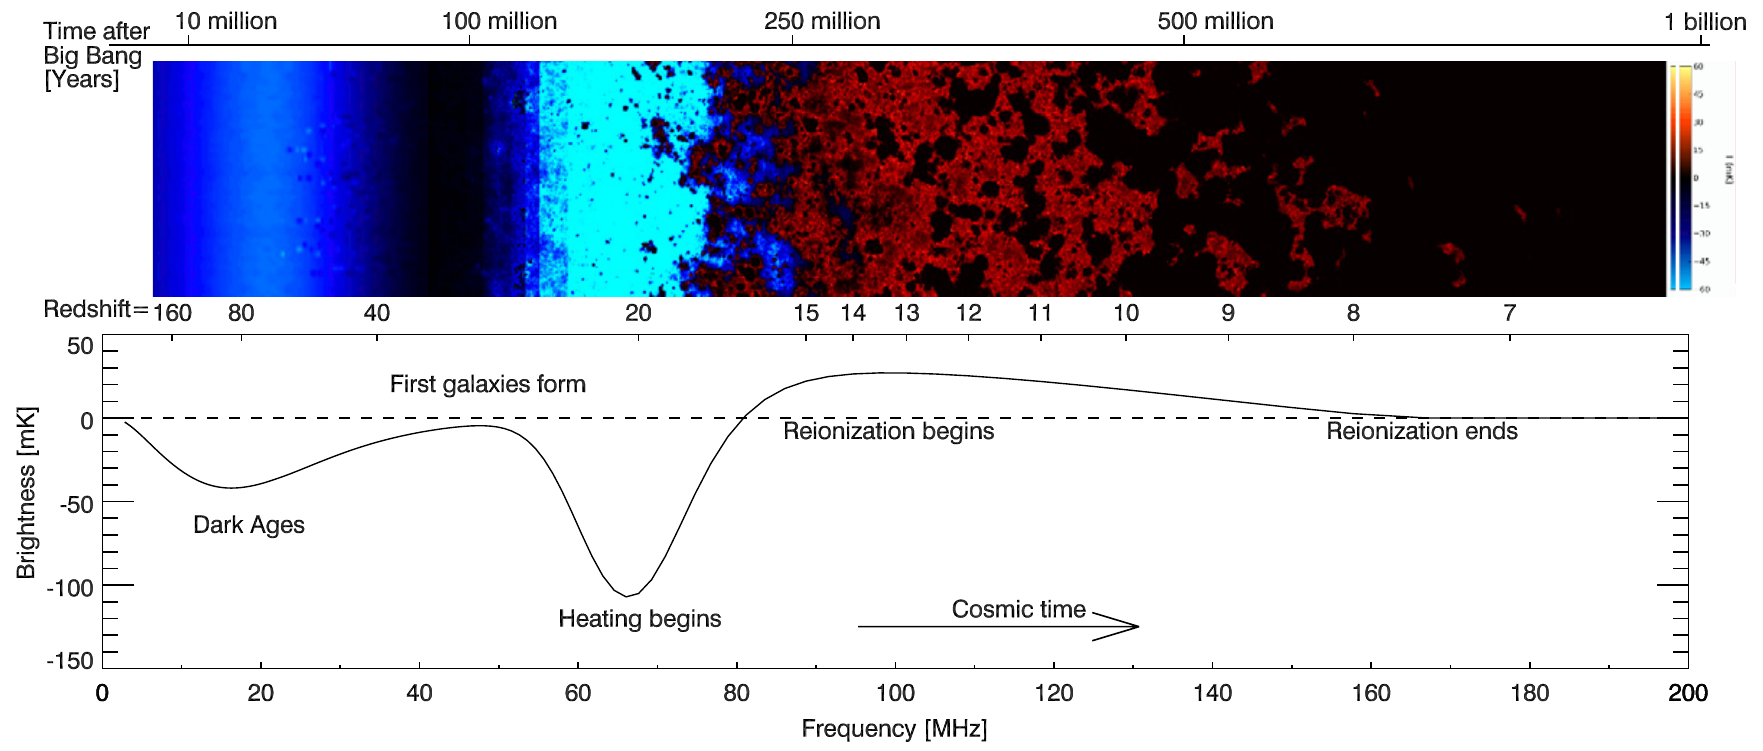
\includegraphics[width=\textwidth]{eor-signal-evolution}
    \caption{EoR 信号的平均强度的演化示意图 (\citeay{pritchard2012})}
  \end{figure}
\end{frame}

%............
\begin{frame}{功率谱}
  \begin{columns}
    \column{0.6\textwidth}
    \begin{itemize}
      \item EoR 信号的频率 $\nu$ 对应于中性氢的视向距离.
      \item EoR 信号的\alert{图像立方} $I(\B{\theta}, \nu)$
        对应于中性氢的三维空间分布.
      \item 通过三维 Fourier 变换,可以从 $I(\B{\theta}, \nu)$
        计算 EoR 信号的\alert{三维功率谱} $P(\B{k})$.
      \item 按一系列球壳对 $P(\B{k})$ 压缩,可得\alert{一维功率谱} $P(k)$.
      \item 按 $k_{\parallel}$ 平面内的一系列圆环压缩,
        得到\alert{二维功率谱} $P(k_{\perp}, k_{\parallel})$.
    \end{itemize}

    \column{0.4\textwidth}
    \begin{figure}
      \centering
      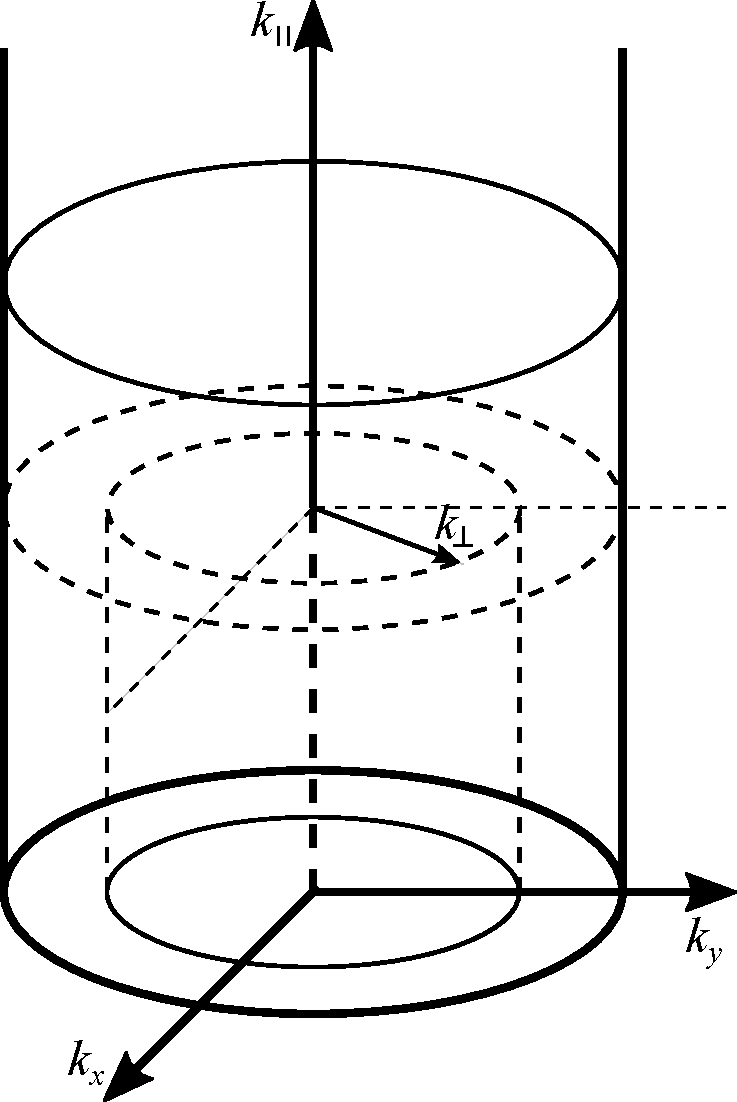
\includegraphics[width=\columnwidth]{ps2d-annuli-diagram}
      \caption{二维功率谱的计算示意图 (\citeay{thyagarajan2013})}
    \end{figure}
  \end{columns}
\end{frame}

%............
\begin{frame}{前景楔形和 EoR 窗口}
  \begin{itemize}
    \item 同一条基线的空间分辨率随频率的增大而提高,
      即所测量的波数正比于频率: $u = b/\lambda \propto \nu$.
      称为\alert{色彩效应 (chromatic effect)}.
    \item 基线越长,色彩效应越显著.
    \item 将 $k_{\perp}$ 模式里的功率\enquote{混合}到 $k_{\parallel}$ 模式里,
      导致\alert{前景楔形} \cite{morales2012}.
  \end{itemize}

  \vspace{-1ex}
  \myfigure{%
    height=0.68\textheight,
    vertcap,
  }{chromatic-baselines}{%
    基线的色彩效应示意图
  }
\end{frame}

%............
\begin{frame}
  \alert{EoR 窗口}边界 \cite{thyagarajan2013}:
  \begin{equation}
    \label{eq:eor-window}
    k_{\parallel} \ge
      \frac{H(z) D_{\!C}(z)}{c (1+z)}
      \left[ k_{\perp} \sin\Phi
        + \frac{2\Cpi \nu_0 w}{(1+z) D_{\!C}(z) B_f} \right] ,
  \end{equation}
  $D_{\!C}(z)$ 为共动距离,$B_f$ 为带宽,$w$ 描述前景漏失程度.

  \vspace{-1ex}
  \myfigure{%
    height=0.8\textheight,
    vertcap,
  }{EoR-window}{%
    EoR 窗口和前景楔形的示意图
  }
\end{frame}


%=====================================================================
\section{低频射电天空的模拟}

%---------------------------------------------------------------------
\subsection{星系团射电晕}

%............
\begin{frame}{射电晕}
  \begin{itemize}
  \item 之前对射电晕的模拟研究不足,而且建模过于简化.
  \item 本文显著地改进了射电晕的建模,充分考虑了射电晕的形成和演化过程:
    \begin{enumerate}
      \item 从 Press--Schechter (PS) 质量函数模拟星系团的质量和红移分布;
      \item 根据扩展 PS 理论模拟每个星系团的并合历史;
      \item 运用湍流再加速模型,计算并合湍流对高能电子的再加速过程;
      \item 求解 Fokker--Planck (FP) 方程,得到高能电子能谱以及射电晕频谱
        的时间演化;
      \item 计算射电晕的性质并生成图像.
    \end{enumerate}
  \end{itemize}
\end{frame}

%............
\begin{frame}{PS 质量函数}
  \begin{columns}
    \column{0.5\textwidth}
    红移 $z$ 时每单位共动体积内质量范围 $[M,\, M+\D{M}]$ 的星系团数目:
    \begin{multline}
      n_{\R{cl}}(M,z) \,\D{M} =
        \sqrt{\frac{2}{\Cpi}} \frac{\langle \rho_0 \rangle}{M}
        \frac{\delta_c(z)}{\sigma^2(M)} \times \\
        \left| \diff{\sigma(M)}{M} \right|
        \exp\!\left[ -\frac{\delta_c^2(z)}{2\sigma^2(M)} \right]
        \,\D{M} ,
    \end{multline}
    $\langle \rho_0 \rangle$ 是当前的宇宙平均密度,
    $\delta_c(z)$ 是暗物质坍缩的临界密度,
    $\sigma(M)$ 是平均质量为 $M$ 的球形区域里的密度涨落值.

    \column{0.5\textwidth}
    \begin{figure}
      \centering
      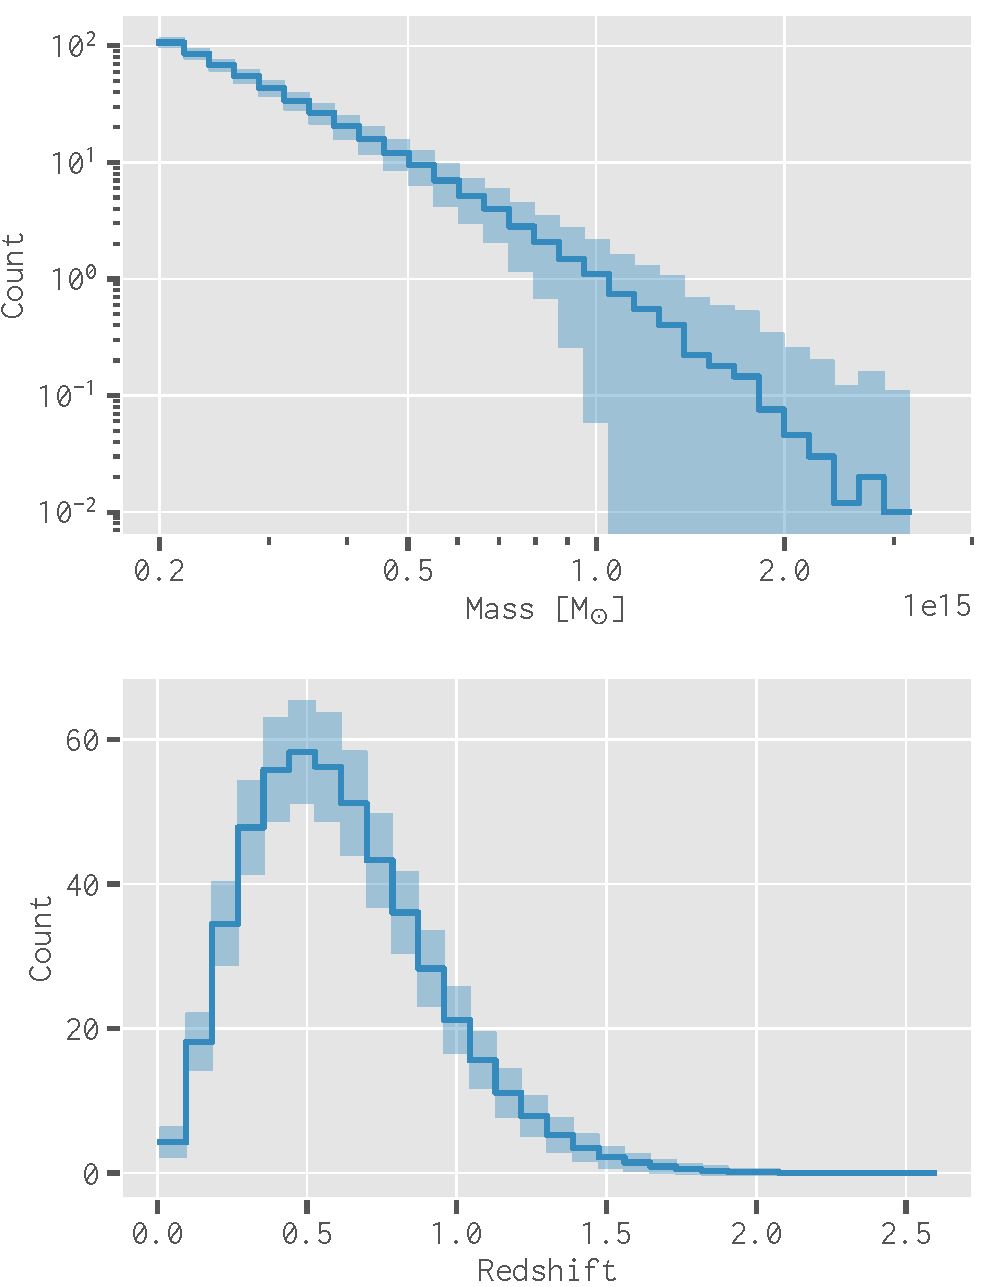
\includegraphics[width=\columnwidth]{mass-z-dist}
      \caption{星系团的红移和质量分布直方图}
    \end{figure}
  \end{columns}
\end{frame}

%............
\begin{frame}{并合历史}
  \begin{columns}
    \column{0.5\textwidth}
    质量为 $M_2$ 的星系团在一个较早时刻 $t_1$ 具有一个质量范围为
    $[M_1,\, M_1+\D{M_1}]$ 的前身的条件概率为:
    \begin{multline}
      \R{Pr}(M_1, t_1 \,|\, M_2, t_2) \,\D{M_1} = \\
        \frac{1}{\sqrt{2\Cpi}} \frac{M_2}{M_1}
        \frac{\delta_{c1} - \delta_{c2}}{(\sigma_1^2 - \sigma_2^2)^{3/2}}
        \left| \diff{\sigma_1^2}{M_1} \right|
        \times \\
        \exp \!\left[ -\frac{(\delta_{c1} - \delta_{c2})^2}
        {2(\sigma_1^2 - \sigma_2^2)} \right] \,\D{M_1} .
    \end{multline}
    利用 Monte Carlo 模拟构建星系团的成长历史,即\alert{并合树}.

    \column{0.5\textwidth}
    \begin{figure}
      \centering
      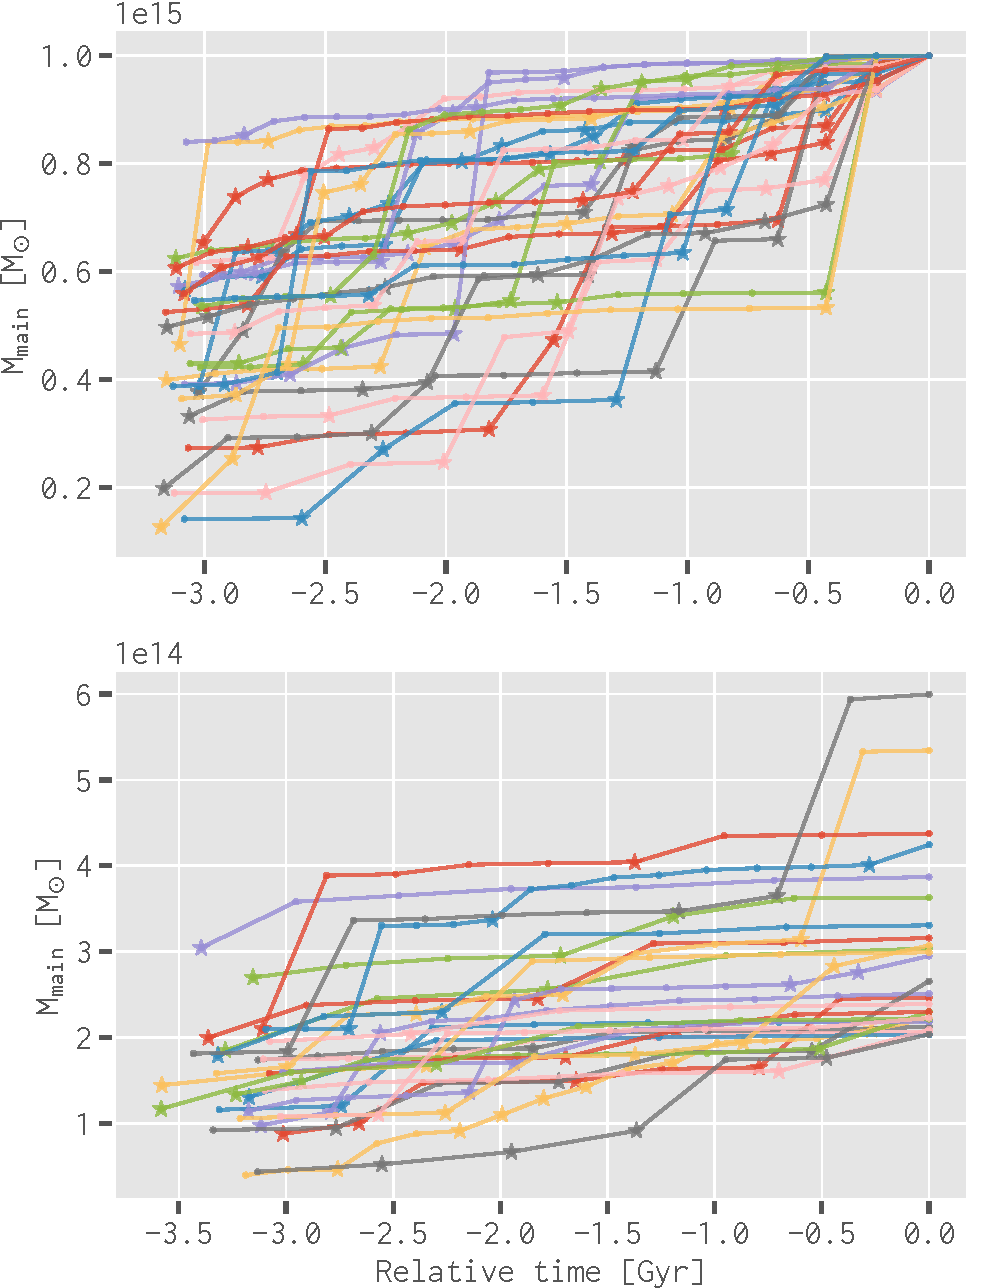
\includegraphics[width=\columnwidth]{merging-history}
      \caption{星系团并合树的模拟结果示例}
    \end{figure}
  \end{columns}
\end{frame}

%............
\begin{frame}{演化模型}
  在湍流加速和能量损失的共同作用下,
  电子能谱 $n_e(\gamma, t)$ 随时间的演化由 \alert{FP 方程}描述:
  \begin{multline}
    \pdiff{n_e(\gamma, t)}{t} =
      \pdiff{}{\gamma} \left[ n_e(\gamma, t) \left(
        \left| \diff{\gamma}{t} \right| -
        \frac{2}{\gamma} D_{\gamma\gamma}(\gamma, t) \right) \right] + \\
      \pdiff{}{\gamma} \left[
      D_{\gamma\gamma} \pdiff{n_e(\gamma, t)}{\gamma} \right]
      + Q_e(\gamma, t) ,
  \end{multline}
  $D_{\gamma\gamma}$ 描述湍流和电子的相对作用,\\
  $|\R{d}\gamma / \R{d}t|$ 是电子的能量损失速率,\\
  $Q_e$ 描述了电子的注入过程.
\end{frame}

%............
\begin{frame}
  \begin{alertblock}{电子注入过程}
    \smallskip
    \begin{itemize}
      \item AGN 活动、恒星形成等过程持续地将初级电子注入 ICM.
      \item 可以假定:
        \begin{itemize}
          \item 注入速率 $K_e$ 恒定;
          \item 注入电子的能谱为幂律形式,谱指数为 $s$;
          \item 注入电子的总能量密度与 ICM 热能密度 $\epsilon_{\R{th}}$
            之比为 $\eta_e$.
        \end{itemize}
      \item 可得:
        \begin{align}
          Q_e(\gamma, t) & = K_e \gamma^{-s} , \\
          K_e & = \frac{(s-2) \eta_e \epsilon_{\R{th}}}{
            \epsilon_e \tau_{\R{cl}}} \gamma_{\R{min}}^{s-2} ,
        \end{align}
        其中 $\epsilon_e = m_e c^2$,
        $\tau_{\R{cl}}$ 为星系团的年龄.
    \end{itemize}
  \end{alertblock}
\end{frame}

%............
\begin{frame}
  \begin{alertblock}{湍流加速}
    \smallskip
    \begin{itemize}
      \item 湍流与 ICM 中的宇宙射线粒子发生作用而耗散能量,
        于是初级电子获得能量被加速 \cite{brunetti2011}.
      \item 该加速机制的扩散系数为 \cite{miniati2015}:
        \begin{equation}
          D_{\gamma\gamma} =
            2 \gamma^2 \zeta k_L
            \frac{\langle (\delta v_t)^2 \rangle^2}{\chi_{\R{cr}} c_s^3} ,
        \end{equation}
        $\zeta$ 为 ICM 等离子体的不稳定性,\\
        $\chi_{\R{cr}}$ 为宇宙射线的能量密度与 ICM 热能密度之比,\\
        $k_L = 2\Cpi / r_{\R{turb}}$ 为湍流注入尺度,
        $c_s$ 为 ICM 中的声速.
      \item $\langle (\delta v_t)^2 \rangle$ 为湍流的速度弥散:
        \begin{equation}
          \langle (\delta v_t)^2 \rangle =
            \langle (\delta v_0)^2 \rangle +
            \frac{2 \eta_t E_m}{M_{\R{turb}}} ,
        \end{equation}
        $\eta_t$ 为并合注入湍流的能量比例.
    \end{itemize}
  \end{alertblock}
\end{frame}

%............
\begin{frame}
  \begin{alertblock}{湍流加速}
    \smallskip
    \begin{itemize}
      \item $E_m$ 为并合释放的能量:
        \begin{equation}
          E_m \simeq \bar{\rho}_m v_{\R{imp}}^2
            \Cpi r_s^2 r_{\R{vir,m}} ,
        \end{equation}
        $\bar{\rho}_m$ 为主团的平均气体密度,
        $v_{\R{imp}}$ 为并合的碰撞速度,\\
        $r_s$ 为子团的剥离半径.
      \item $r_{\R{turb}}$ 为湍流区域的半径:
        \begin{equation}
          r_{\R{turb}} \simeq r_s + r_{\R{c,m}}
            = r_s + 0.1\,r_{\R{vir,m}} .
        \end{equation}
      \item $M_{\R{turb}}$ 为湍流区域内的气体质量:
        \begin{equation}
          M_{\R{turb}} =
            \int_0^{r_{\R{turb}}} \! \rho(r) \,4\Cpi r^2 \,\D{r} ,
        \end{equation}
        $\rho(r)$ 为已并合星系团的气体密度轮廓,由 $\beta$ 模型描述.
    \end{itemize}
  \end{alertblock}
\end{frame}

%............
\begin{frame}
  \begin{alertblock}{能量损失}
    \smallskip
    \begin{itemize}
      \item 与 CMB 光子发生逆 Compton 散射:
        \begin{equation}
          \left( \diff{\gamma}{t} \right)_{\R{IC}} =
            \num{-4.32e-4} \,\gamma^2 (1+z)^4
            \quad [\si{\per\Gyr}] .
        \end{equation}
      \item 同步辐射:
        \begin{equation}
          \left( \diff{\gamma}{t} \right)_{\R{syn}} =
            \num{-4.10e-5} \,\gamma^2
            \left( \frac{B}{\SI{1}{\uG}} \right)^2
            \quad [\si{\per\Gyr}] .
        \end{equation}
      \item 与 ICM 热电子发生 Coulomb 碰撞:
        \begin{multline}
          \left( \diff{\gamma}{t} \right)_{\R{Coul}} =
            \num{-3.79e4} \left( \frac{n_{\R{th}}}{\SI{1}{\per\cm\cubed}} \right)
            \left[ 1 + \frac{1}{75} \ln \left(
              \gamma\,\frac{\SI{1}{\per\cm\cubed}}{n_{\R{th}}} \right) \right]
            \\ \quad [\si{\per\Gyr}] ,
        \end{multline}
        $n_{\R{th}}$ 为热电子数密度.
    \end{itemize}
  \end{alertblock}
\end{frame}

%............
\begin{frame}{数值实现}
  \begin{itemize}
    \item 采用 \citeay{chang1970} 提出的有限差分法求解 FP 方程.
    \item 初始电子能谱 $n_e(\gamma, t_0)$:
      让积累的电子能谱 $\tilde{n}_e(\gamma) = Q_e(\gamma) \tau_0$
      在无并合的情况下演化 \SI{1}{\Gyr}.
    \item 每次并合的有效加速时间:
      \begin{equation}
        \tau_{\R{turb}} \simeq 2 r_{\R{turb}} / v_{\R{imp}} .
      \end{equation}
    \item 同步辐射发射率:
      \begin{equation}
        J_{\R{syn}}(\nu) =
          \frac{\sqrt{3} \,e^3 B}{m_e c^2}
          \!\int_{\gamma_{\R{min}}}^{\gamma_{\R{max}}}
          \!\!\!\int_0^{\Cpi/2}
          \! F_{\R{syn}} \!\left( \frac{\nu}{\nu_c} \right)
          n_e(\gamma, t) \sin^2 \!\theta \,\D{\theta} \,\D{\gamma} ,
      \end{equation}
      $\theta$ 为电子的螺距角,
      $\nu_c$ 为电子的临界频率,\\
      $F_{\R{syn}}()$ 是同步辐射核函数.
  \end{itemize}
\end{frame}

%............
\begin{frame}{识别和大小}
  \begin{itemize}
    \item 只有活跃的湍流加速,射电晕才能形成.
    \item 判别射电晕在频率 $\nu$ 处存在的两点依据:
      \begin{itemize}
        \item 同步辐射发射率 $J_{\R{syn}}(\nu)$
          是相应的\enquote{参考值} $J'_{\R{syn}}(\nu)$ 的至少 1000 倍;
        \item 同步辐射在该频率处的谱指数 $\alpha_{\nu} \le 3$.
      \end{itemize}

    \item 射电晕的半径 $r_{\R{halo}}$ 随星系团的维里半径 $r_{\R{vir}}$
      超线性地增大,据此假定:
      \begin{equation}
        r_{\R{halo}} = f_r R_{\R{turb}}
          \left( \frac{r_{\R{vir}}}{r_{\R{vir,*}}} \right)^b ,
      \end{equation}
      $R_{\R{turb}}$ 是最大湍流区域的半径,\\
      $r_{\R{vir,*}}$ 是质量为 \SI{e15}{\solarmass} 的参考星系团的维里半径.
    \item 对比观测的标度关系 \cite{cassano2007},
      选取 $f_r = 0.7$ 和 $b = 1.8$.
  \end{itemize}
\end{frame}

%............
\begin{frame}
  \begin{figure}
    \centering
    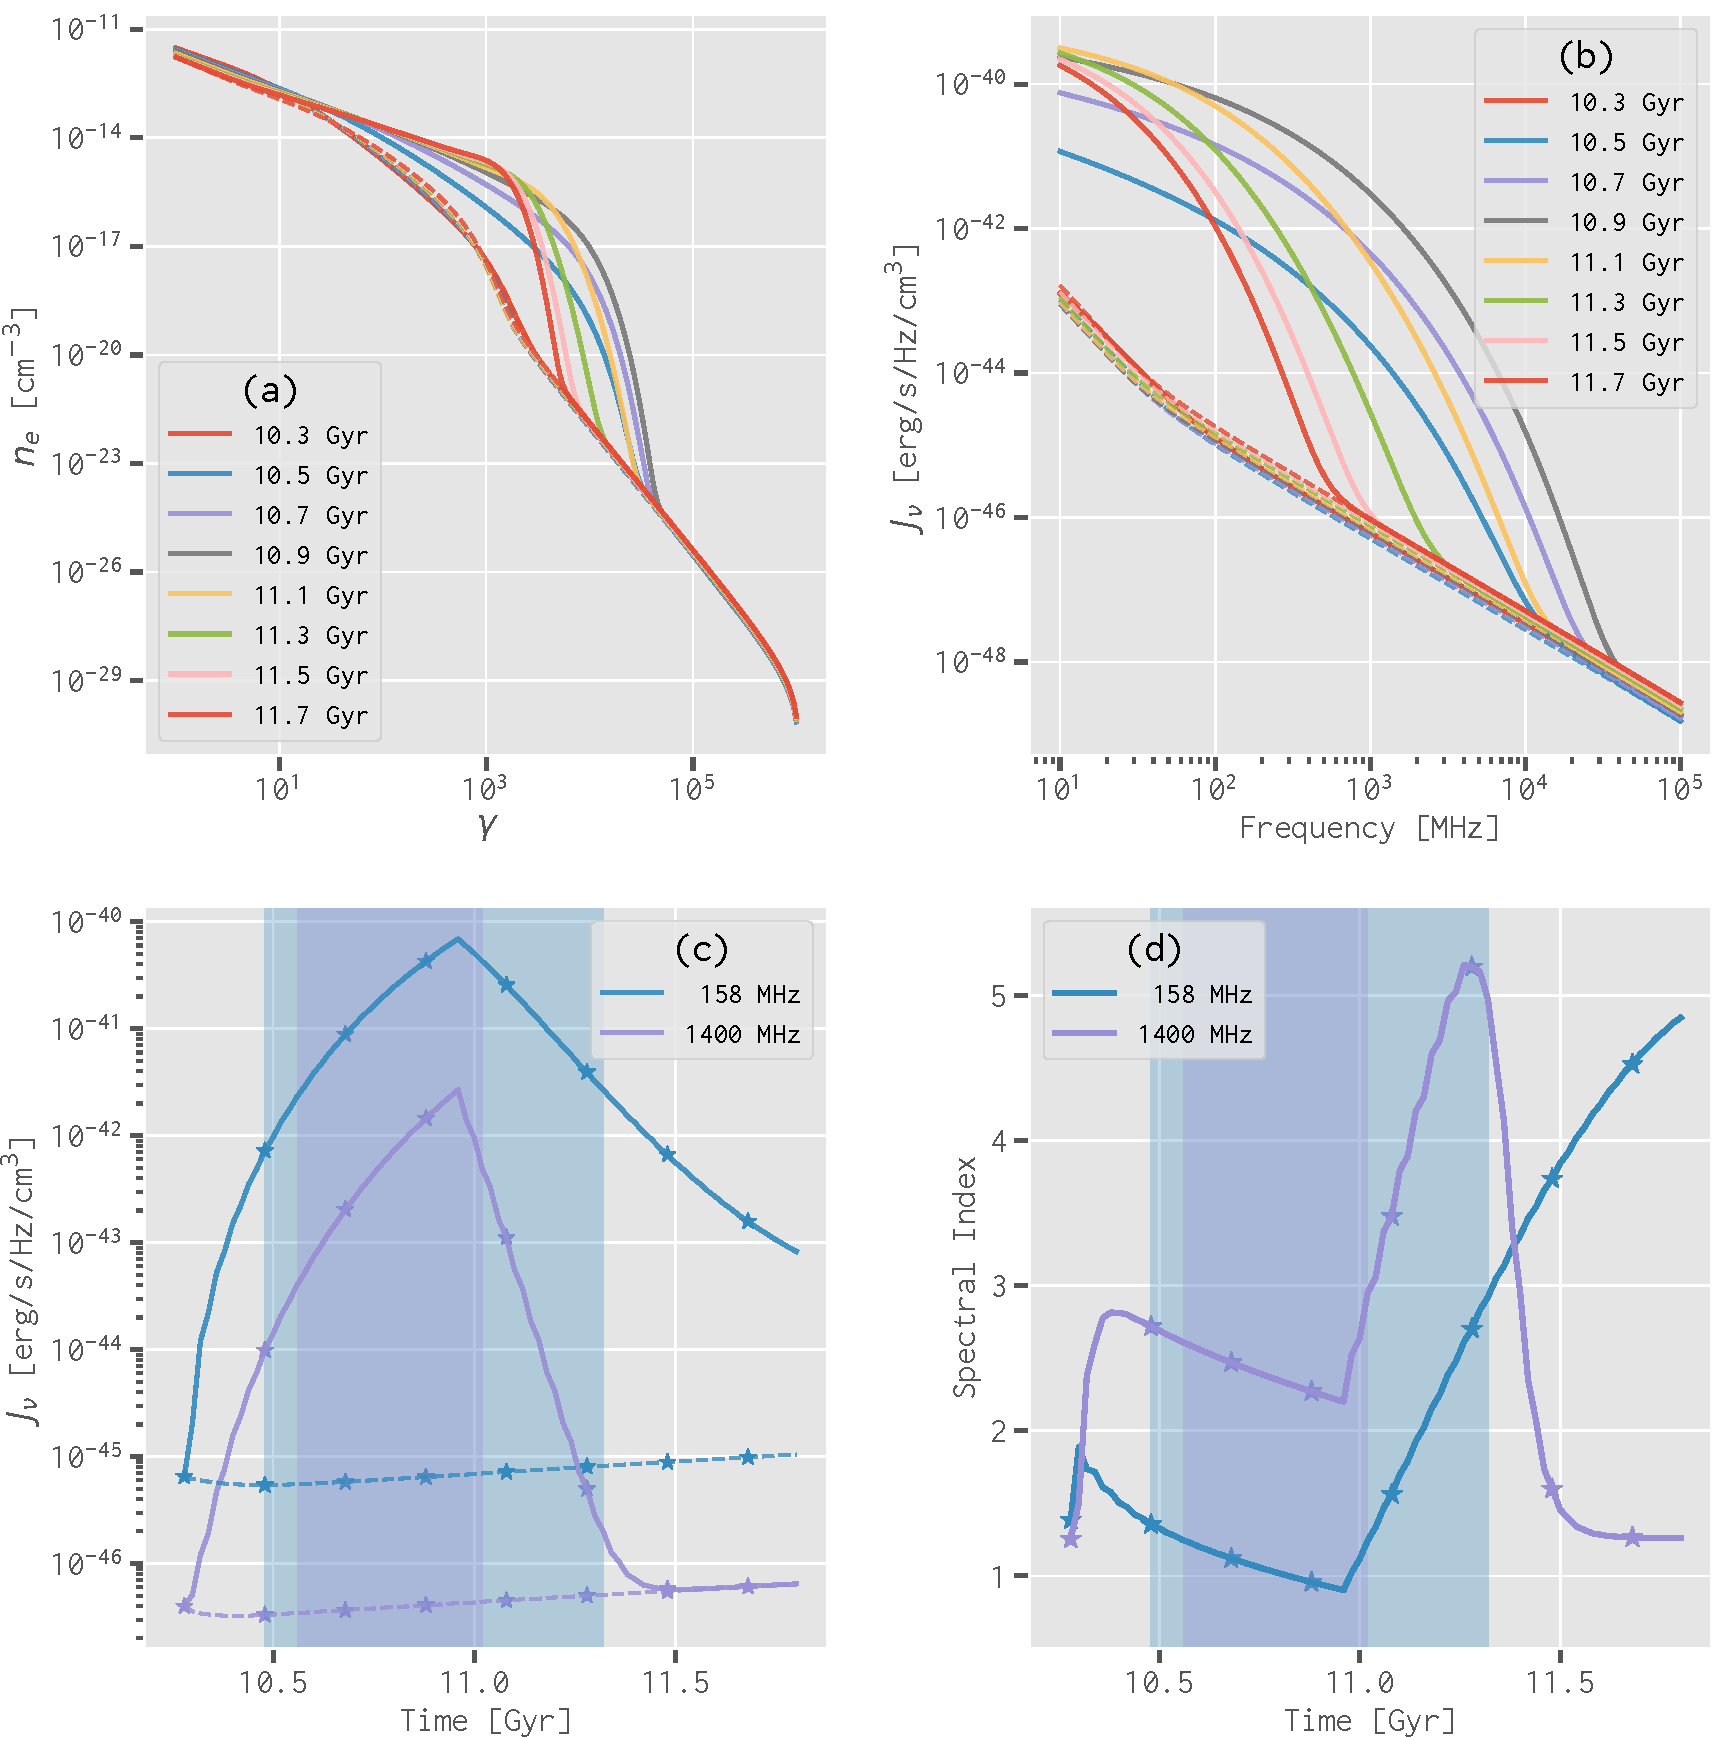
\includegraphics[width=0.9\textwidth]{spec-evo-example}
    \caption{电子能谱和同步辐射频谱随时间的演化示例}
  \end{figure}
\end{frame}

%............
\begin{frame}{模型参数调节}
  \begin{itemize}
    \item 射电晕模型的 5 个待调节参数:
      \begin{itemize}
        \item $\eta_e$:
          注入电子的总能量密度与 ICM 热能密度 $\epsilon_{\R{th}}$ 之比;
        \item $\eta_t$:
          并合释放的能量中转化为湍流能量的比例;
        \item $\chi_{\R{cr}}$:
          宇宙射线的能量密度与 ICM 热能密度 $\epsilon_{\R{th}}$ 之比;
        \item $\chi_{\R{turb}}$:
          初  始湍流的能量密度与 ICM 热能密度 $\epsilon_{\R{th}}$ 之比;
        \item $\zeta$:
          ICM 等离子体的不稳定性参数.
      \end{itemize}
    \item 对比观测结果:
      \begin{itemize}
        \item 射电晕 \SI{1.4}{\GHz} 功率 ($P_{1400}$)
          与星系团质量 ($M_{\R{vir}}$) 的标度关系;
        \item 射电晕 \SI{1.4}{\GHz} 流量函数.
      \end{itemize}
    \item 最终选取参数:
      $\eta_e = 0.01\%$,
      $\eta_t = 15\%$,
      $\chi_{\R{cr}} = 1.5\%$,
      $\chi_{\R{turb}} = 1.5\%$,
      $\zeta = 0.1$.
  \end{itemize}
\end{frame}

%............
\begin{frame}{建模结果}
  \begin{columns}
    \column{0.5\textwidth}
    \begin{figure}
      \centering
      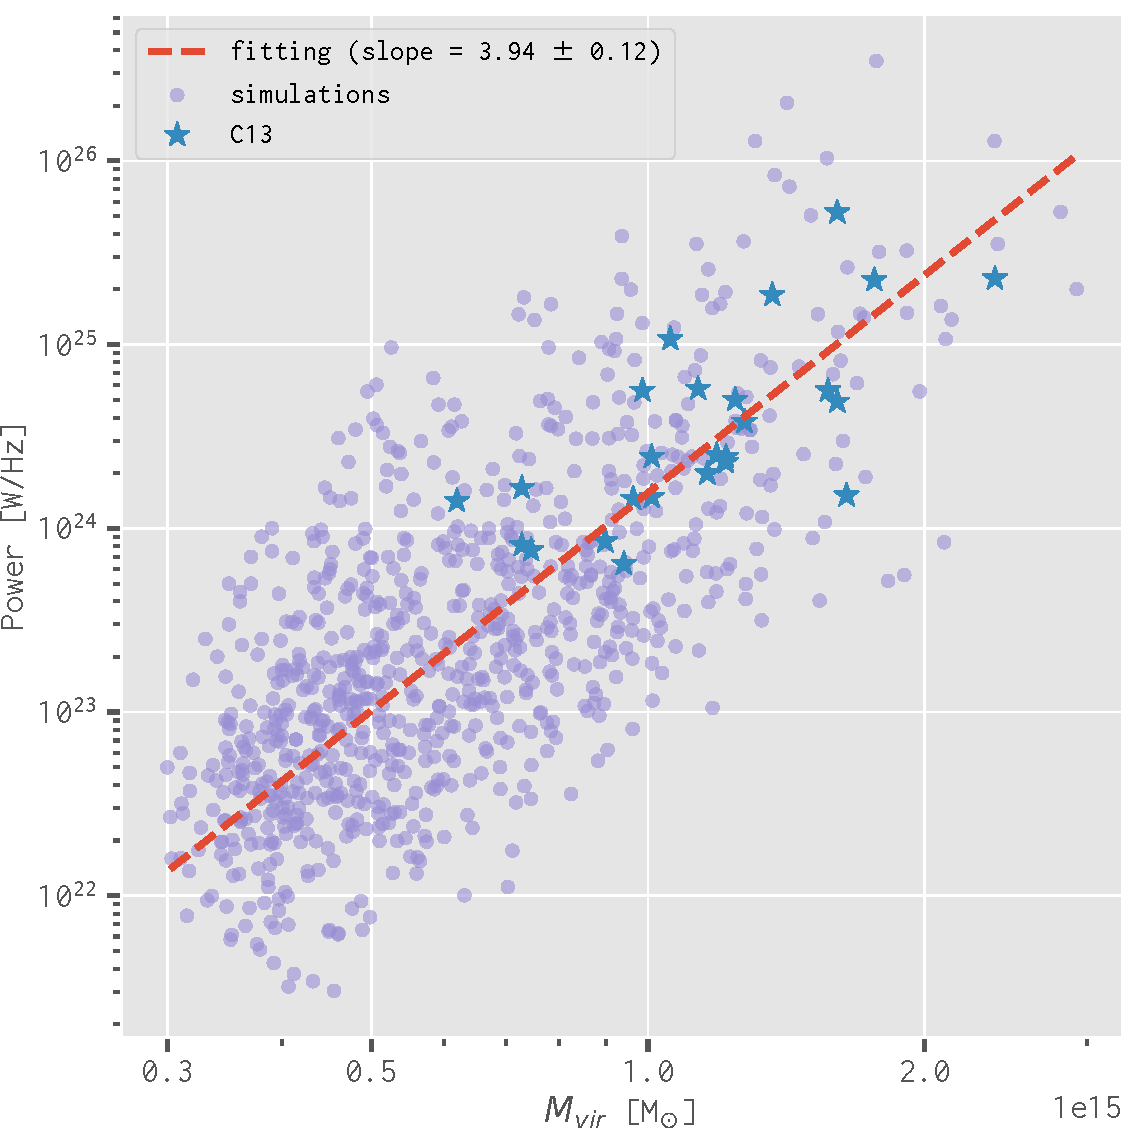
\includegraphics[width=\columnwidth]{halo-power-mvir}
      \caption{$P_{1400}$--$M_{\R{vir}}$ 标度关系的对比}
    \end{figure}

    \column{0.5\textwidth}
    \begin{figure}
      \centering
      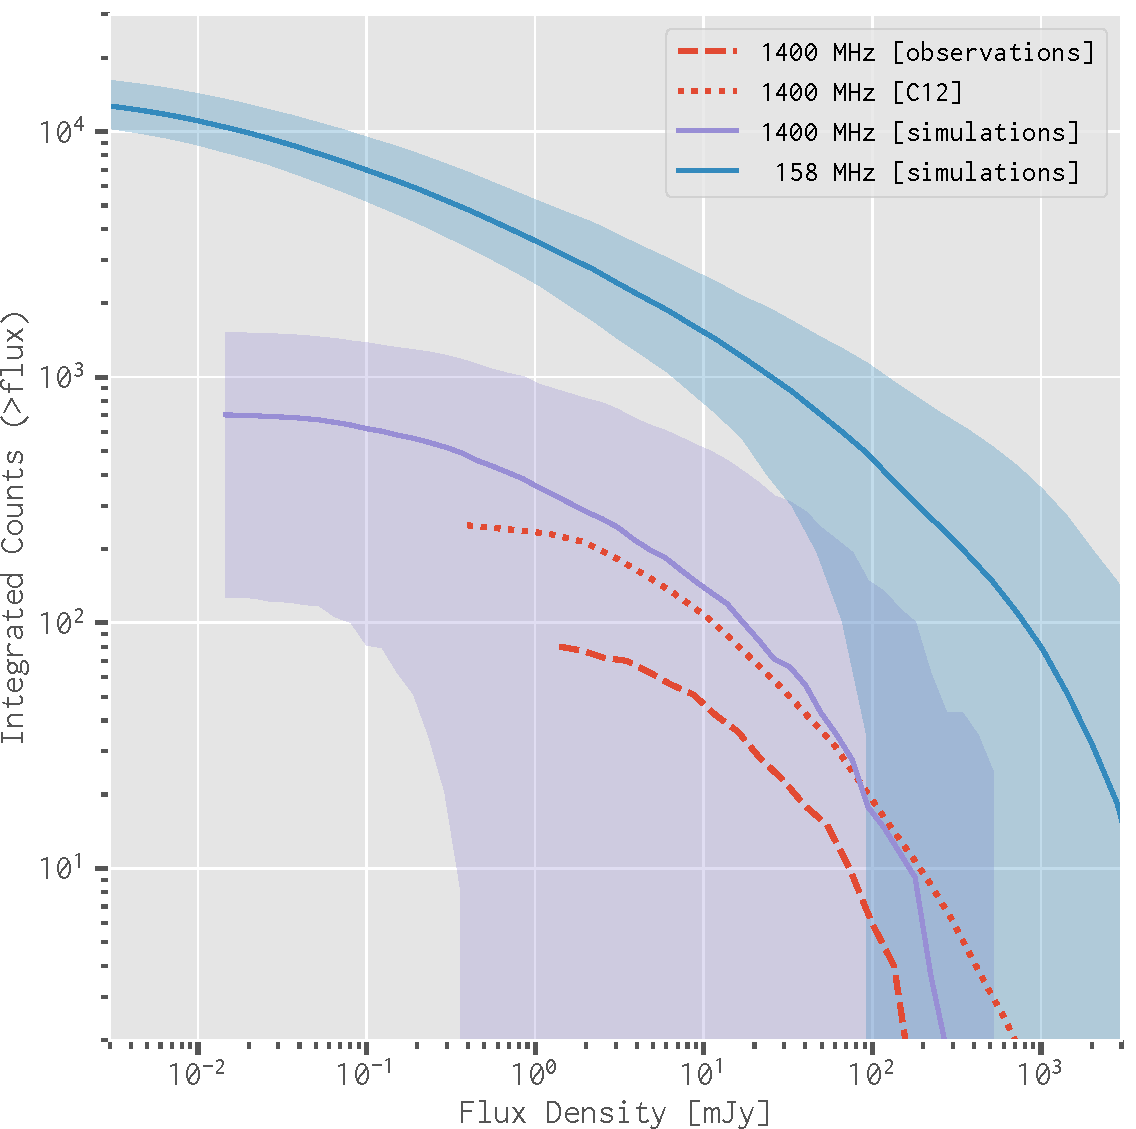
\includegraphics[width=\columnwidth]{fluxfunc-simucomp}
      \caption{\SI{1.4}{\GHz} 流量函数的对比}
    \end{figure}
  \end{columns}
\end{frame}

%............
\begin{frame}{图像生成}
  \begin{itemize}
    \item 射电晕在频率 $\nu$ 处的功率和流量密度:
      \begin{align}
        P_{\R{halo}}(\nu)
          & = \frac{4\Cpi}{3} r^3_{\R{halo}} J_{\R{syn}}(\nu) , \\
        S_{\R{halo}}(\nu)
          & = \frac{(1+z_{\R{sim}}) P_{\R{halo}}[\nu (1+z_{\R{sim}})]}{
            4\Cpi D^2_{\!L}(z_{\R{sim}})} ,
      \end{align}
      $D_{\!L}$ 是光度距离,因子 $(1+z_{\R{sim}})$ 为 $K$ 修正.
    \item 采用指数型轮廓来描述射电晕的角向平均亮度分布:
      \begin{equation}
        I_{\nu}(\theta) = I_{\nu,0} \exp
          \left( -\frac{3\theta}{\theta_{\R{halo}}} \right) ,
      \end{equation}
      $\theta = r / D_{\!A}(z_{\R{sim}})$ 为角半径,
      $I_{\nu,0}$ 为中心亮度.
    \item 利用 Rayleigh--Jeans 近似,得到亮温度分布图像.
    \item 为了考虑亮射电晕在不同天区的显著涨落,重复模拟 100 次射电晕.
  \end{itemize}
\end{frame}

%---------------------------------------------------------------------
\subsection{其他前景成分}

%............
\begin{frame}{银河系同步辐射}
  \begin{itemize}
    \item 以 Haslam \SI{408}{\MHz} 巡天图\cite{haslam1982} 为模板,
      按幂律谱形式外延:
      \begin{equation}
        T_b^{\R{syn}}(\hat{\B{r}}, \nu)
          = T_b^{\R{haslam}}(\hat{\B{r}})
            \left( \frac{\nu}{\SI{408}{\MHz}}
            \right)^{-\alpha_{\R{syn}}(\hat{\B{r}})} .
      \end{equation}
    \item $T_b^{\R{haslam}}(\hat{\B{r}})$
      为银河系 $\hat{\B{r}}$ 处的 \SI{408}{\MHz} 亮温度;\\
      使用了 \citeay{remazeilles2015} 重新处理的全天图.
    \item $\alpha_{\R{syn}}(\hat{\B{r}})$ 为同步辐射谱指数;\\
      使用了 \citeay{giardino2002} 处理的谱指数全天分布图.
  \end{itemize}
\end{frame}

%............
\begin{frame}{银河系自由--自由辐射}
  \begin{itemize}
    \item 自由–自由辐射和 Hα 辐射源自相同的辐射区域,两者之间存在紧密联系.
    \item Hα 辐射易被尘埃吸收,需要进行修正:
      \begin{equation}
        I_{\R{Hα}}^{\R{corr}}(\hat{\B{r}})
          = I_{\R{Hα}}(\hat{\B{r}}) \times
            10^{0.0185 \, f_d \, D(\hat{\B{r}})} ,
      \end{equation}
      $D(\hat{\B{r}})$ 是尘埃柱密度分布图 \cite{schlegel1998},\\
      $f_d$ 是尘埃在视线方向上的有效吸收比例.
    \item 在频率 $\nu$ 处的自由--自由辐射:
      \begin{equation}
        T_b^{\R{ff}}(\hat{\B{r}}, \nu)
          = 38.86 \,\nu^{-2.1} 10^{(290/T_e)} \, T_e^{0.667} \,a(\nu, T_e)
            \left[ \frac{I_{\R{Hα}}^{\R{corr}}(\hat{\B{r}})}{\si{\rayleigh}}
            \right] \quad [\si{\kelvin}] ,
      \end{equation}
    \item $a(\nu, T_e)$ 是光深的修正因子:
      \begin{equation}
        a(\nu, T_e) =
          0.183 \,\nu^{0.1} T_e^{-0.15}
          \left[ 3.91 - \ln \nu + 1.5 \ln T_e \right] .
      \end{equation}
    \item 本文取 $f_d = 0.33$ 和 $T_e = \SI{7000}{\kelvin}$
      \cite{dickinson2003}.
  \end{itemize}
\end{frame}

%............
\begin{frame}{河外点源}
  \begin{itemize}
    \item 继承自我们之前的一项工作: \citeay{wang2010}
    \item 模拟了下述 4 类点源:
      \begin{enumerate}
        \item 恒星形成星系
        \item 射电宁静 AGN
        \item FR I 型和 II 型 AGN
        \item GHz 倒转谱和致密陡谱 AGN
      \end{enumerate}
    \item 第 1--3 类点源的模拟使用了 \citeay{wilman2008} 针对 SKA 的模拟结果.
    \item 第 4 类点源的模拟使用了相应的光度函数和频谱模型.
  \end{itemize}
\end{frame}

%............
\begin{frame}[c]{}
  \hfill
  \rotatebox{90}{射电晕}
  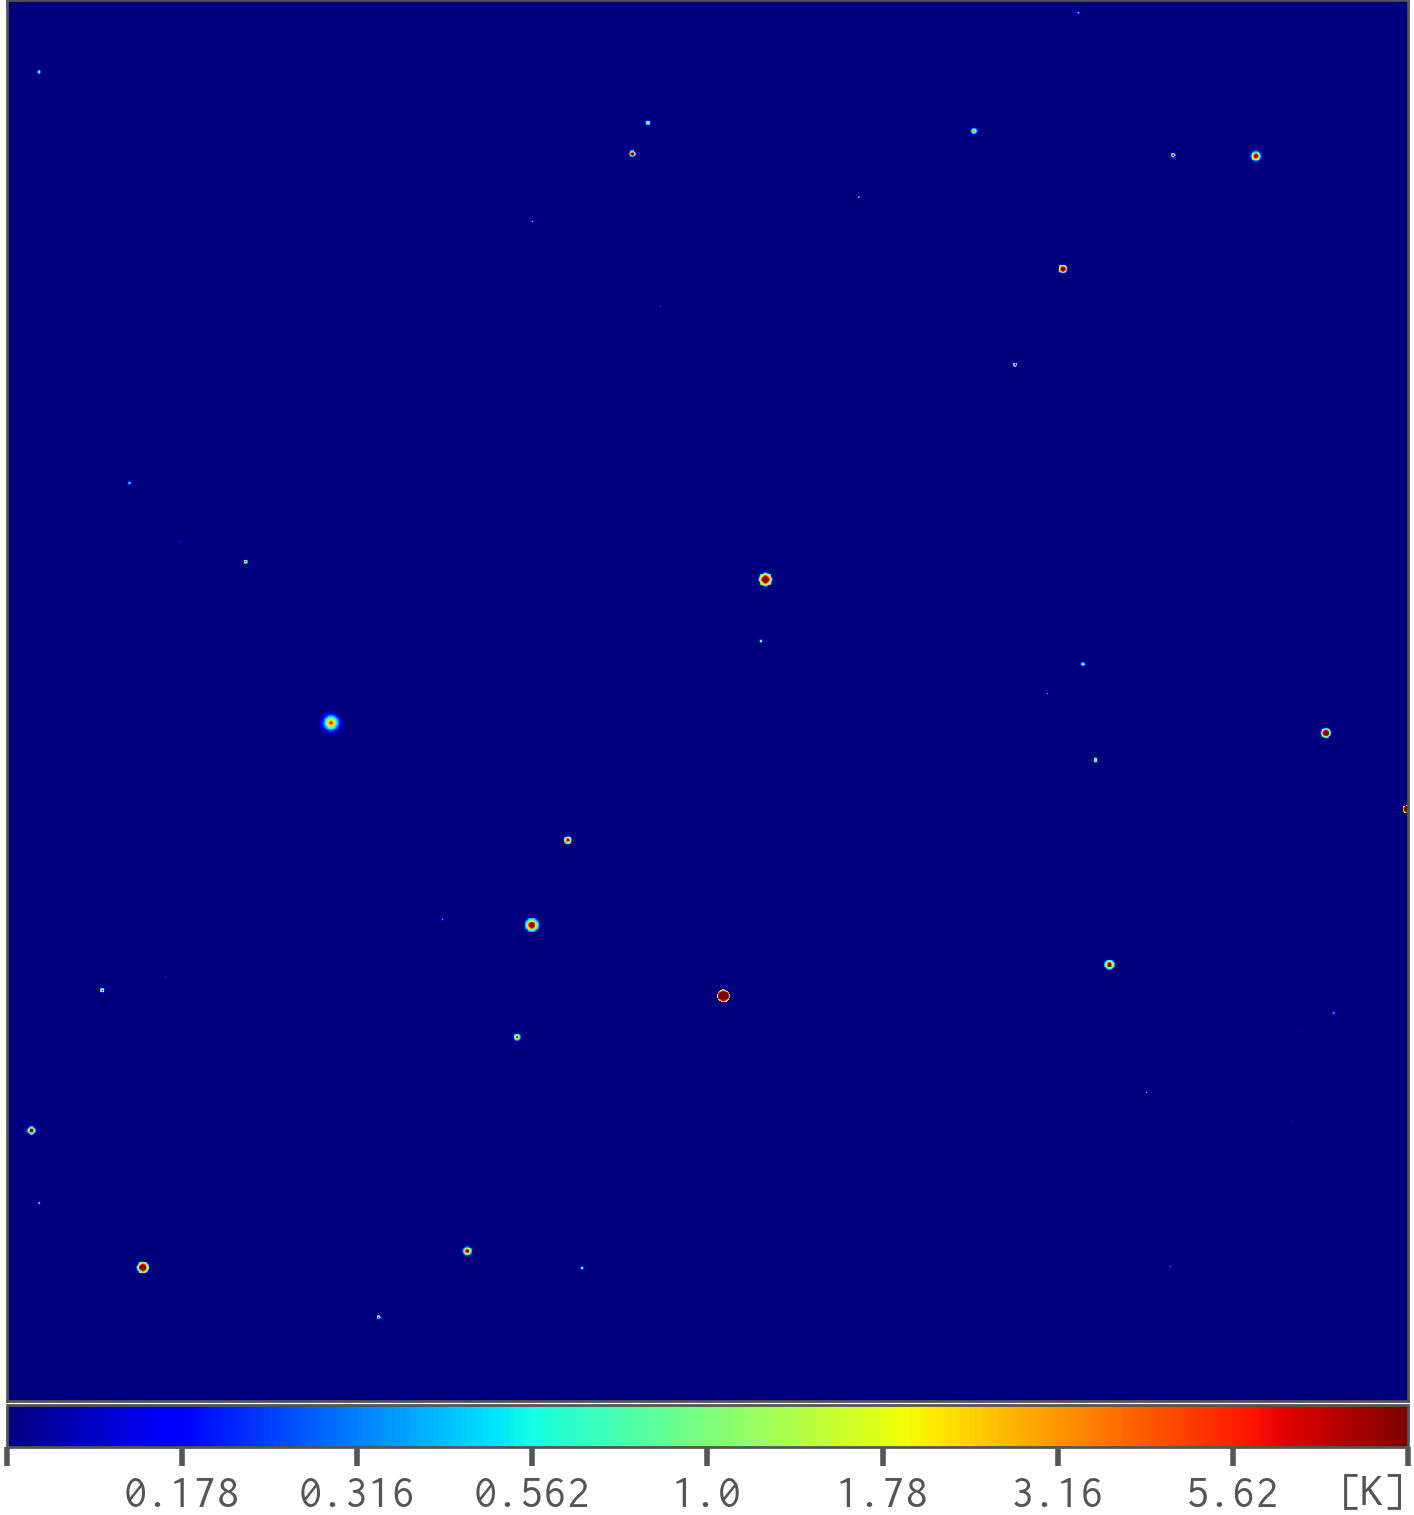
\includegraphics[height=0.55\textheight]{skymap-halos-f158}
  \hspace{1em}
  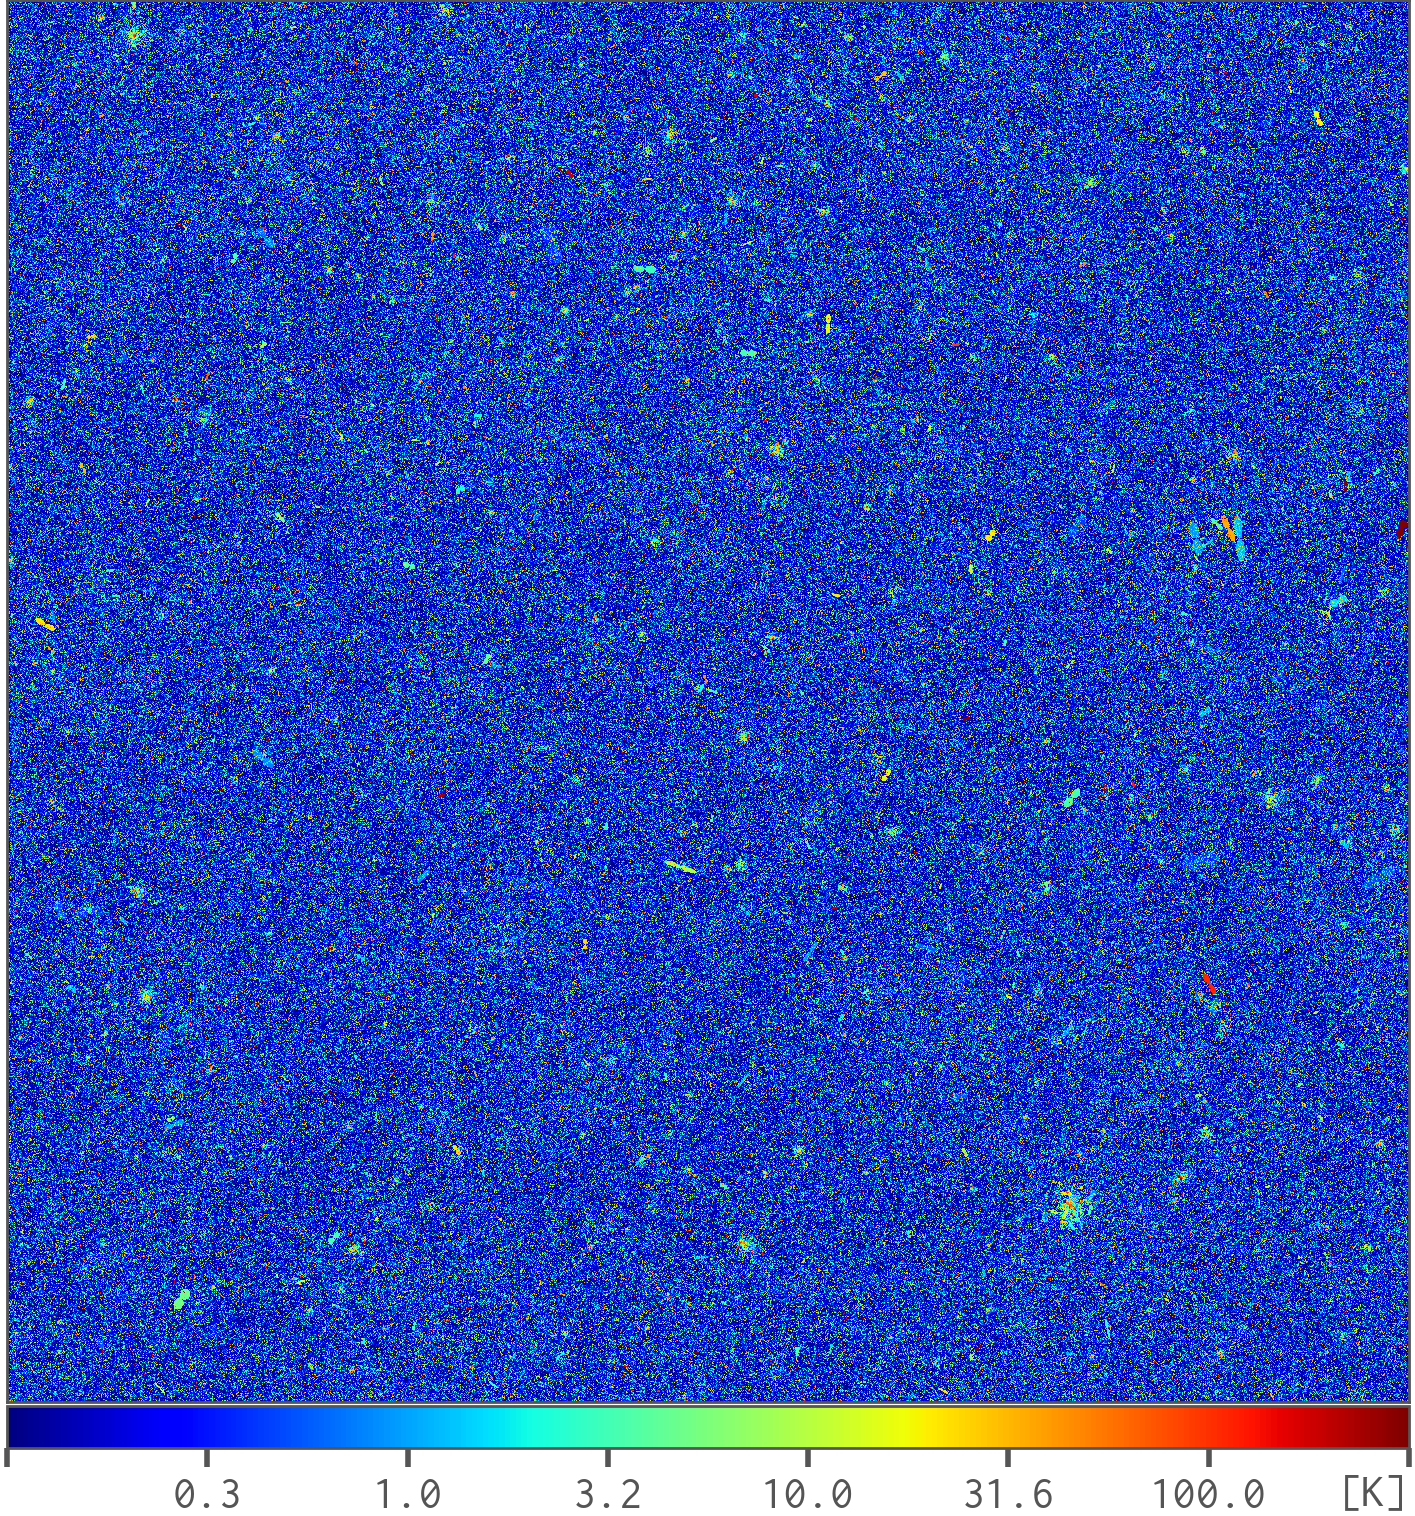
\includegraphics[height=0.55\textheight]{skymap-ptrsrc-f158}
  \rotatebox{90}{河外点源}
  \hfill \\
  \hfill
  \rotatebox{90}{银河系同步辐射}
  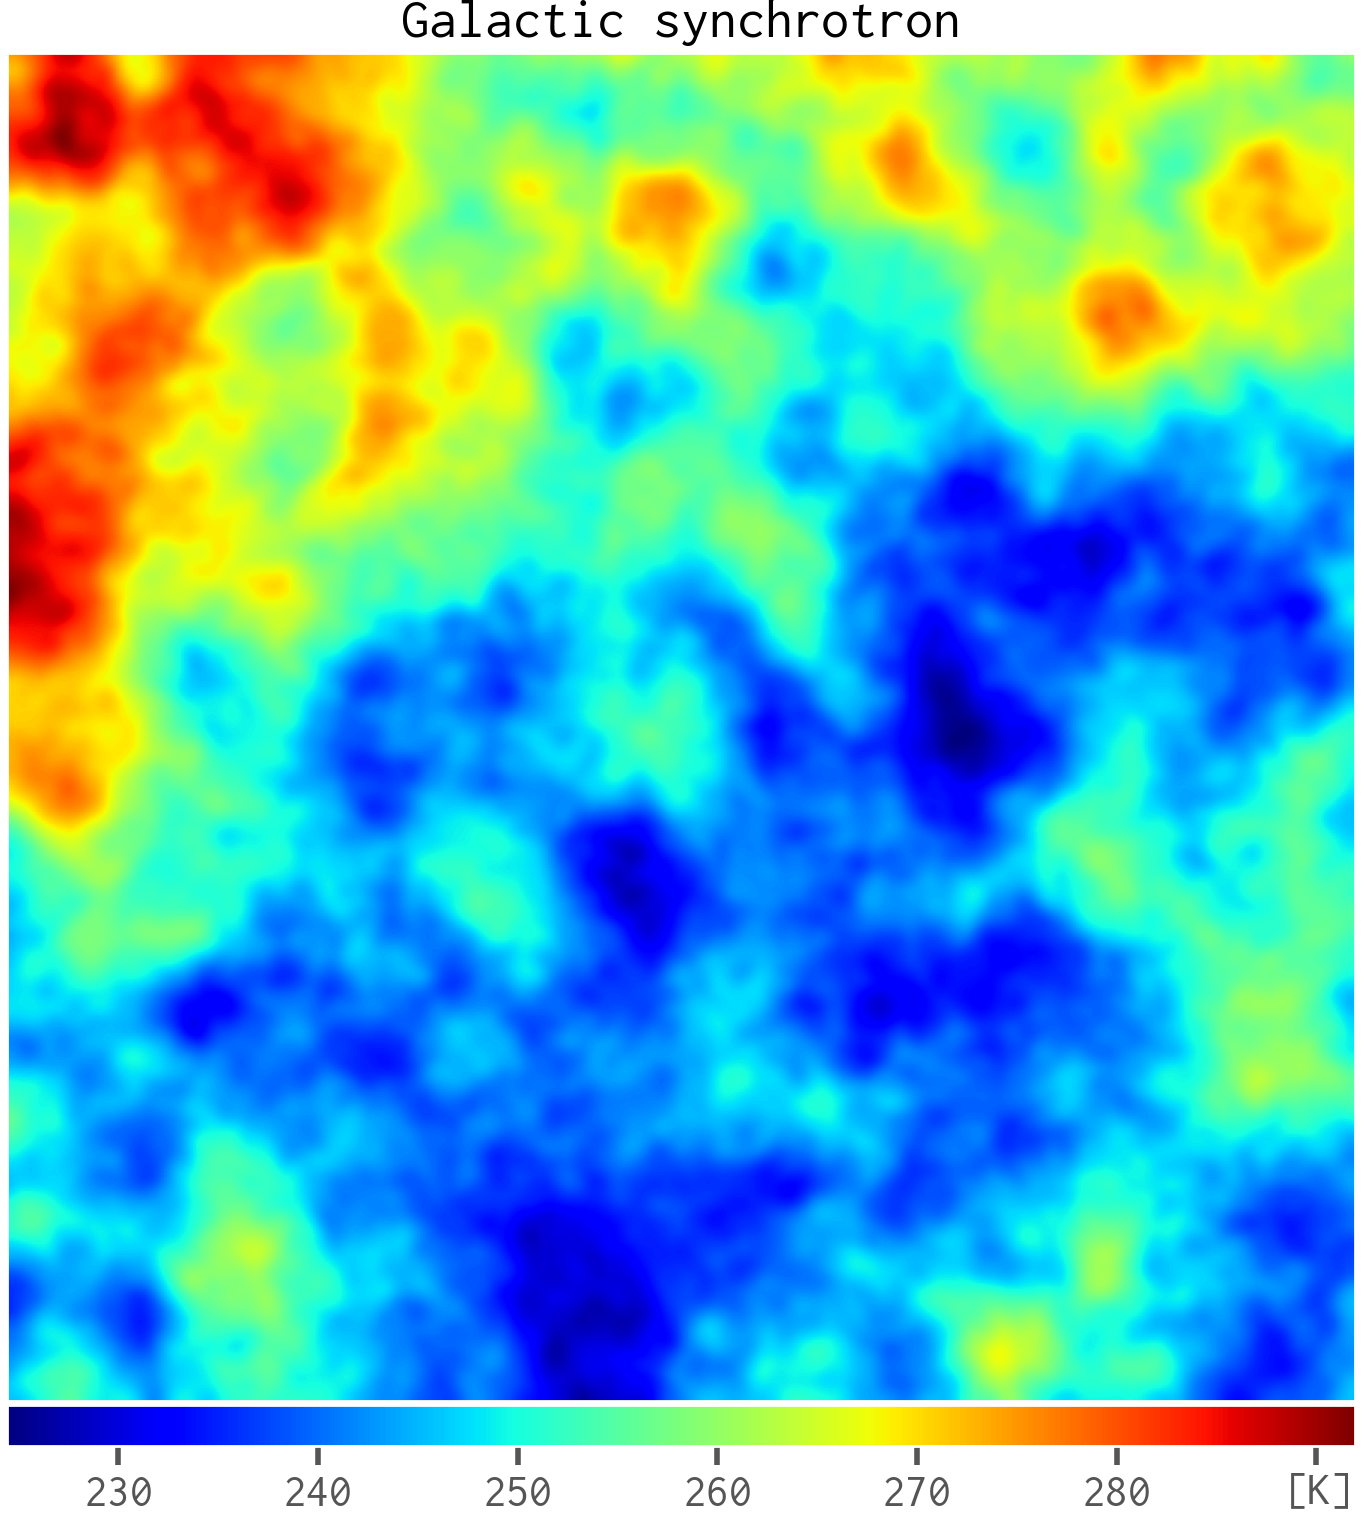
\includegraphics[height=0.55\textheight]{skymap-gsyn-f158}
  \hspace{1em}
  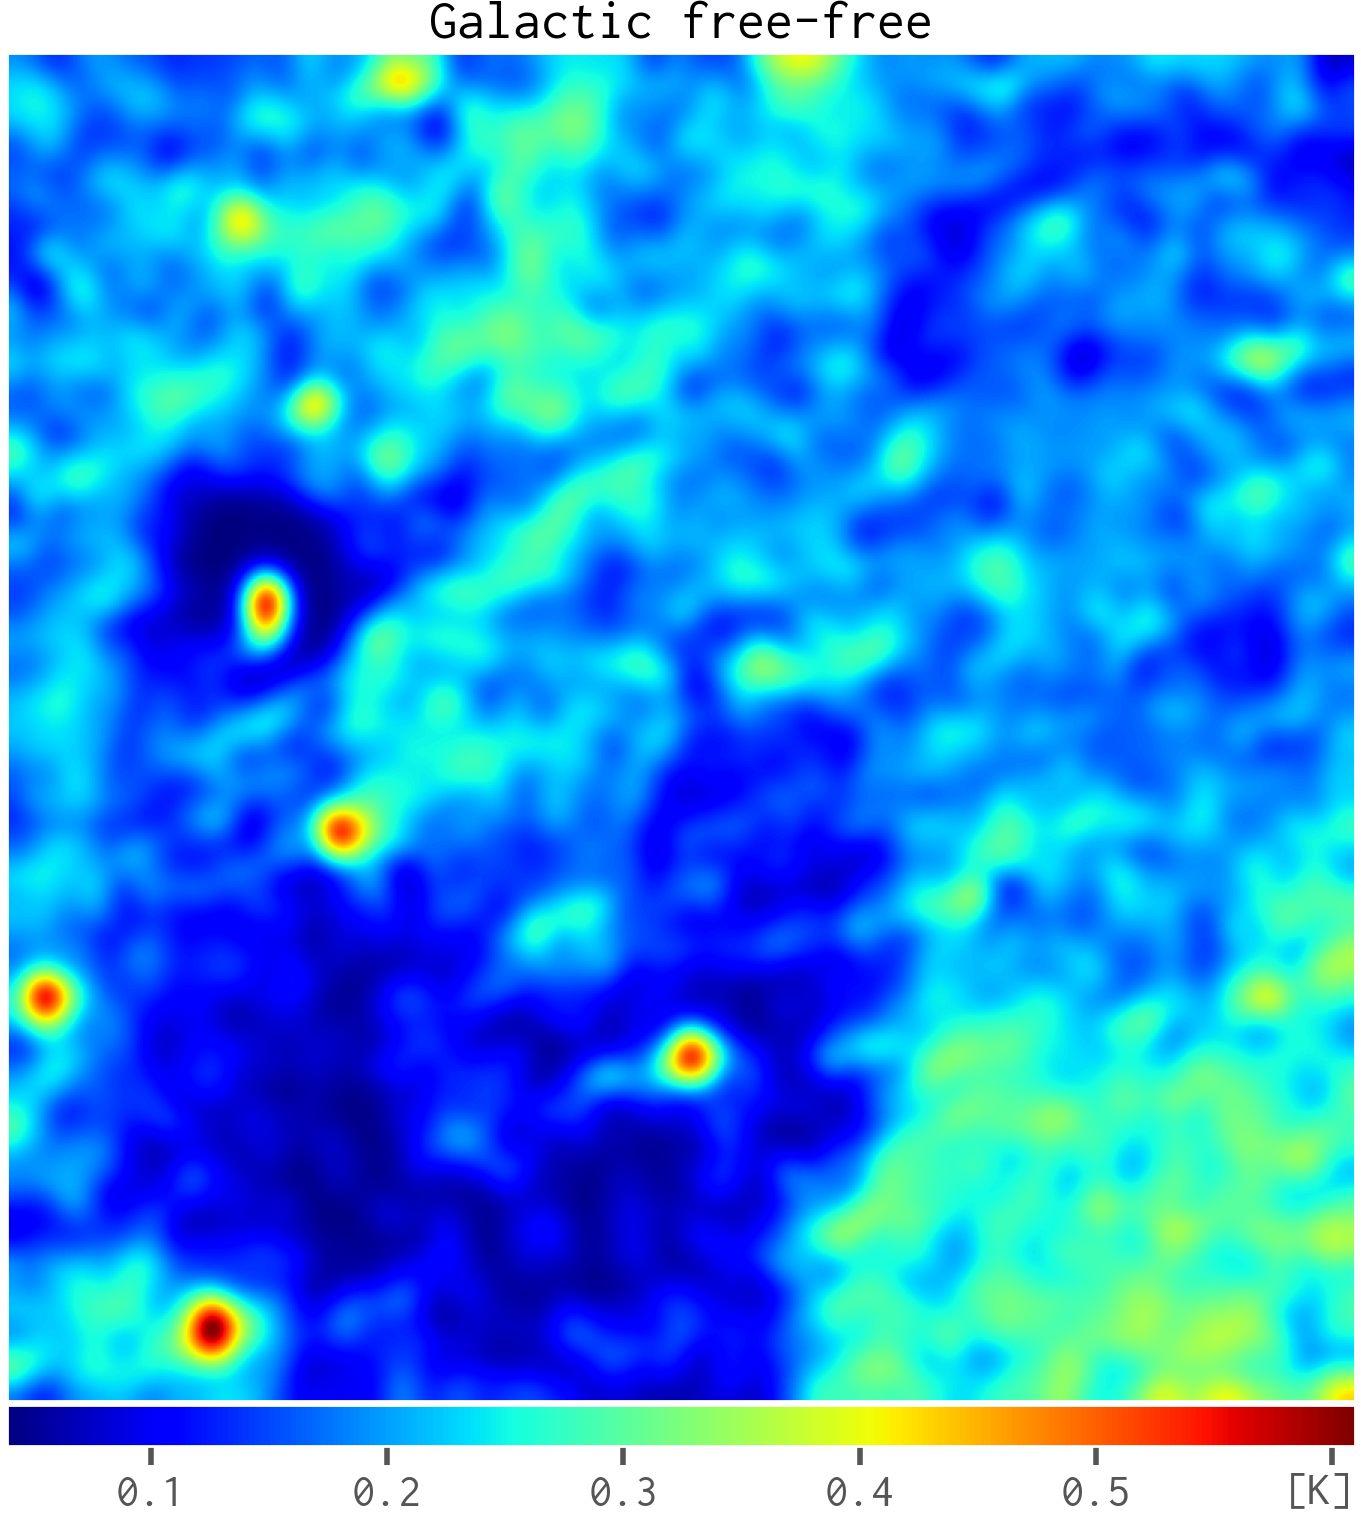
\includegraphics[height=0.55\textheight]{skymap-gff-f158}
  \rotatebox{90}{银河系自由--自由辐射}
  \hfill
\end{frame}

%---------------------------------------------------------------------
\subsection{EoR 信号}

%............
\begin{frame}{EoR 信号}
  \begin{columns}
    \column{0.5\textwidth}
    \begin{itemize}
      \item 使用了 \enquote{Evolution of 21\,cm Structure}
        项目公开的 EoR 模拟数据.
      \item 从推荐的 \enquote{faint galaxies} 情形的光锥图像立方,
        提取所需红移(即频率)处的图像切片.
      \item 经过平铺和缩放处理,与前景天图的大小和分辨率一致.
    \end{itemize}

    \column{0.5\textwidth}
    \begin{figure}
      \centering
      \includegraphics[width=\columnwidth]{skymap-eor-f158}
      \caption{EoR 信号在 \SI{158}{\MHz} 的天图}
    \end{figure}
  \end{columns}
\end{frame}

%---------------------------------------------------------------------
\subsection{干涉阵列的模拟观测}

%............
\begin{frame}{观测模拟}
  \begin{itemize}
    \item 采用目前最新的 SKA1-Low~阵列布局.
    \item 使用 \texttt{OSKAR} 对每张天图进行模拟观测,积分时间 \SI{6}{\hour}.
    \item 观测中心坐标为 (\SI{0}{\degree}, \SI{-27}{\degree}),
      该点能够经过 SKA1-Low 的天顶.
    \item 银河系的同步辐射和自由--自由辐射被叠加在一起.
    \item 假定 \SI{158}{\MHz} 流量密度 $S_{158} > \SI{50}{\mJy}$
      的点源已被移除.
  \end{itemize}
\end{frame}

%............
\begin{frame}{成像}
  \begin{itemize}
    \item 使用 \texttt{WSClean} 从模拟的可见度数据生成\enquote{观测}图像.
    \item 采用 Briggs 权重 \cite{briggs1995},稳健参数设为 0;\\
      兼顾噪声水平和空间分辨率.
    \item 启用联合通道解卷积技术,保证 CLEAN 成分的频谱光滑性.
    \item 只切取图像质量较好的中央区域.
  \end{itemize}
\end{frame}

%............
\begin{frame}{图像立方}
  \begin{itemize}
    \item 频带: 120--128, 154--162, 192--200 MHz
    \item 带宽: \SI{8}{\MHz}
    \item 频率分辨率: \SI{160}{\kHz}
    \item 天区大小: \SI{10 x 10}{\degree}
    \item 图像大小: \num{1800 x 1800}
    \item 像素大小: \SI{20}{\arcsec}
    \item 模拟结果:
      \begin{itemize}
        \item EoR 信号
        \item 射电晕(100 次模拟)
        \item 银河系弥散辐射(包括同步辐射和自由–自由辐射)
        \item 河外点源
      \end{itemize}
  \end{itemize}
\end{frame}


%=====================================================================
\section{射电晕对 EoR 探测的影响}

%............
\begin{frame}{一维功率谱}
  \begin{itemize}
    \item 在 $\SI{0.1}{\per\Mpc} < k < \SI{2}{\per\Mpc}$ 尺度范围内,
      射电晕在三个频带内的典型功率分别是 EoR 信号的功率的
      \num{e4}、\num{e3}、\num{e2.5} 倍.
    \item 在 68\% 的误差范围内,射电晕的功率可变化约 \numrange{10}{100} 倍.
  \end{itemize}

  \begin{figure}
    \centering
    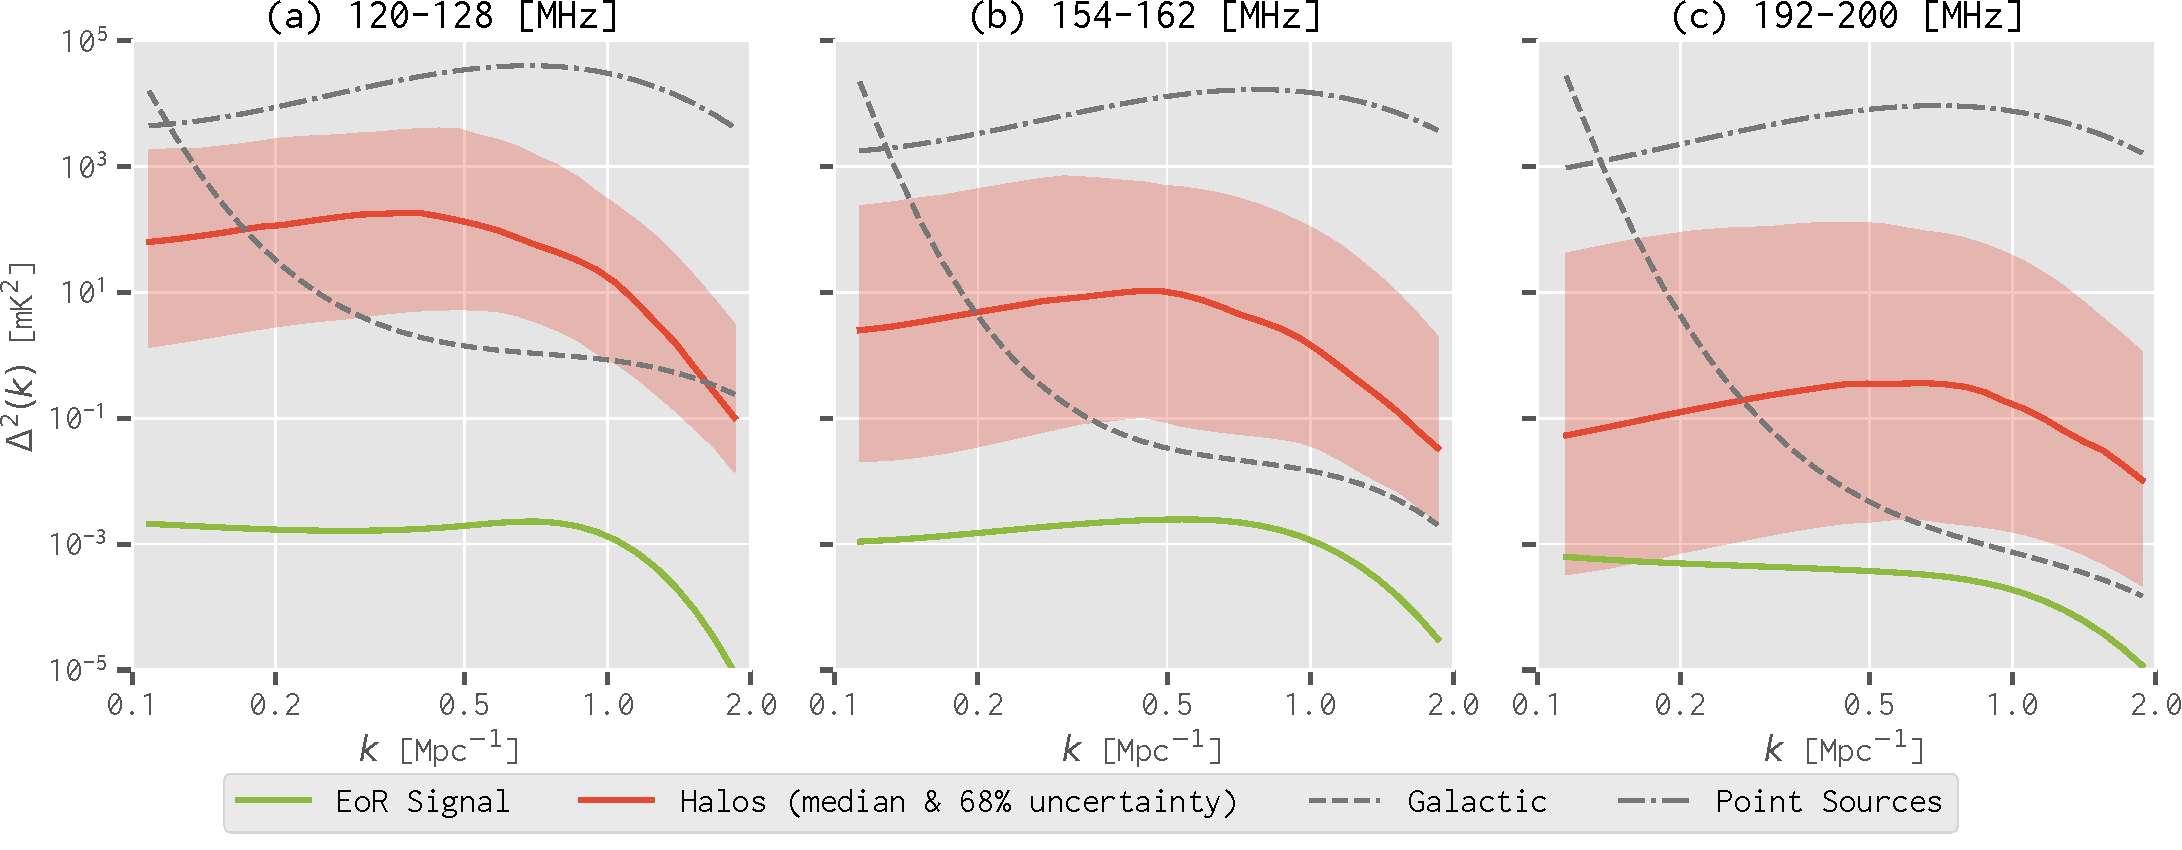
\includegraphics[width=\textwidth]{ps1d-3bands}
    \caption{各成分的一维功率谱对比}
  \end{figure}
\end{frame}

%............
\begin{frame}{二维功率谱}
  \vspace{-1ex}
  \myfigure{%
    height=0.9\textheight,
    %vertcap,
  }{ps2d-band158}{%
    各成分在 \SIrange{154}{162}{\MHz} 频带的二维功率谱对比
  }
\end{frame}

%............
\begin{frame}{二维功率谱之比}
  \begin{itemize}
    \item 射电晕的污染区域呈明显的楔形.
    \item 射电晕在三个频带内的显著污染范围分别约为: \\
      $k_{\perp} \gtrsim \SI{0.1}{\per\Mpc}$、
      $k_{\perp} \gtrsim \SI{0.3}{\per\Mpc}$、
      $k_{\perp} \gtrsim \SI{0.5}{\per\Mpc}$.
    \item 射电晕在较低频率 ($\sim$\,\SI{120}{\MHz}) 的污染程度更强.
  \end{itemize}

  \begin{figure}
    \centering
    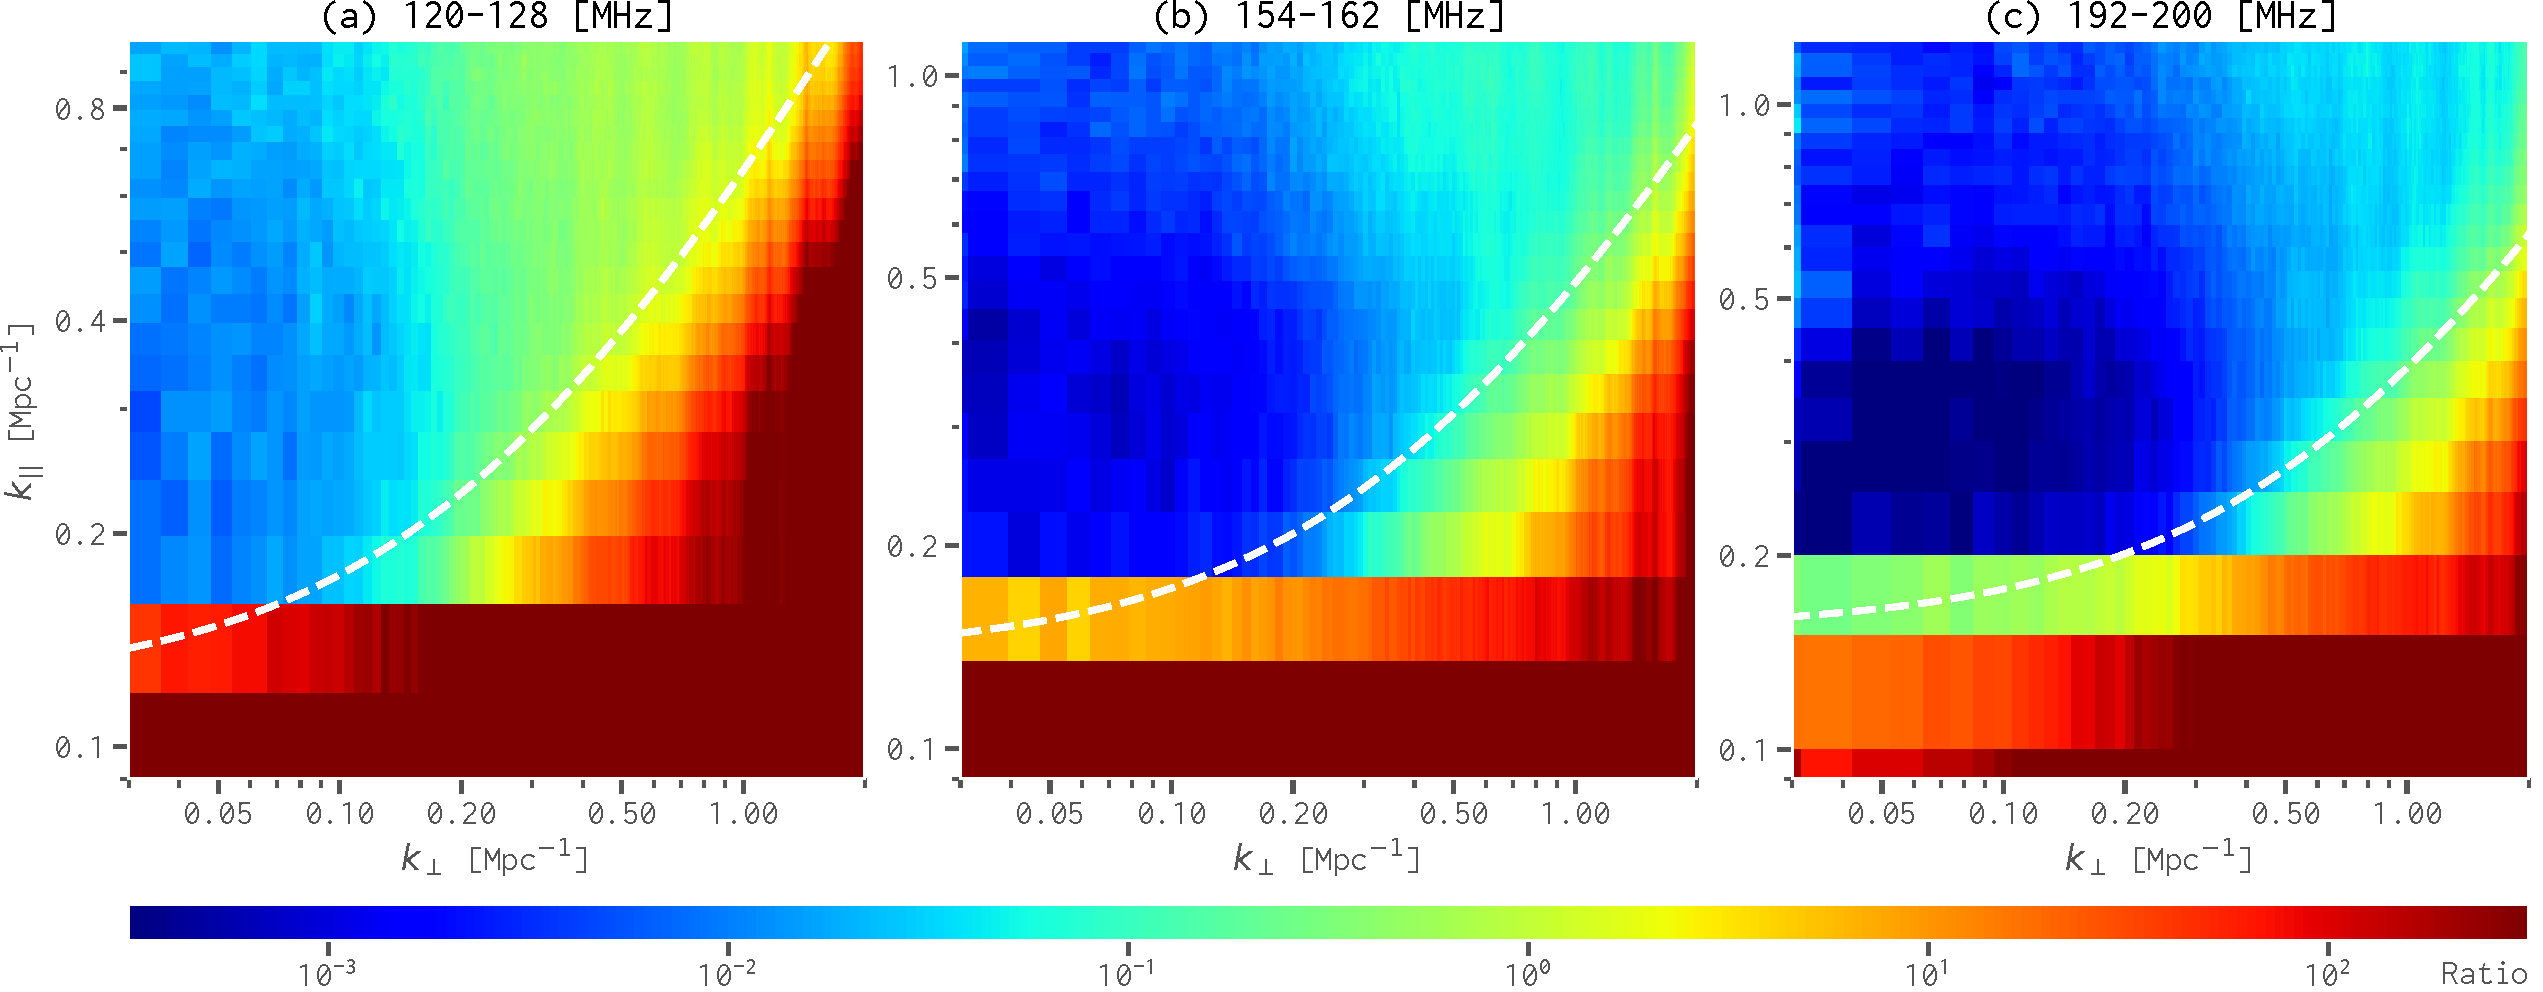
\includegraphics[width=\textwidth]{ps2d-ratio-3bands}
    \caption{射电晕和 EoR 信号的二维功率谱之比}
  \end{figure}
\end{frame}

%............
\begin{frame}{EoR 窗口内的一维功率比}
  \begin{columns}
    \column{0.5\textwidth}
    \begin{itemize}
      \item 选取合适的 EoR 窗口边界 (式~\ref{eq:eor-window}):
        $w = 3$, $\Phi = 1.5$\,FoV.
      \item 损失的 EoR 信号功率比例分别约为: 45\%、46\%、60\%.
      \item 在 $\SI{0.5}{\per\Mpc} < k < \SI{1}{\per\Mpc}$ 尺度范围内,
        EoR 窗口内的一维功率比在 68\% 的误差范围内分别达到约:
        230--800\%、18--95\%、7-40\%.
      \item 射电晕泄漏到 EoR 窗口内的功率仍然可能是显著的,
        尤其在较低频率 ($\sim$\,\SI{120}{\MHz}).
    \end{itemize}

    \column{0.5\textwidth}
    \begin{figure}
      \centering
      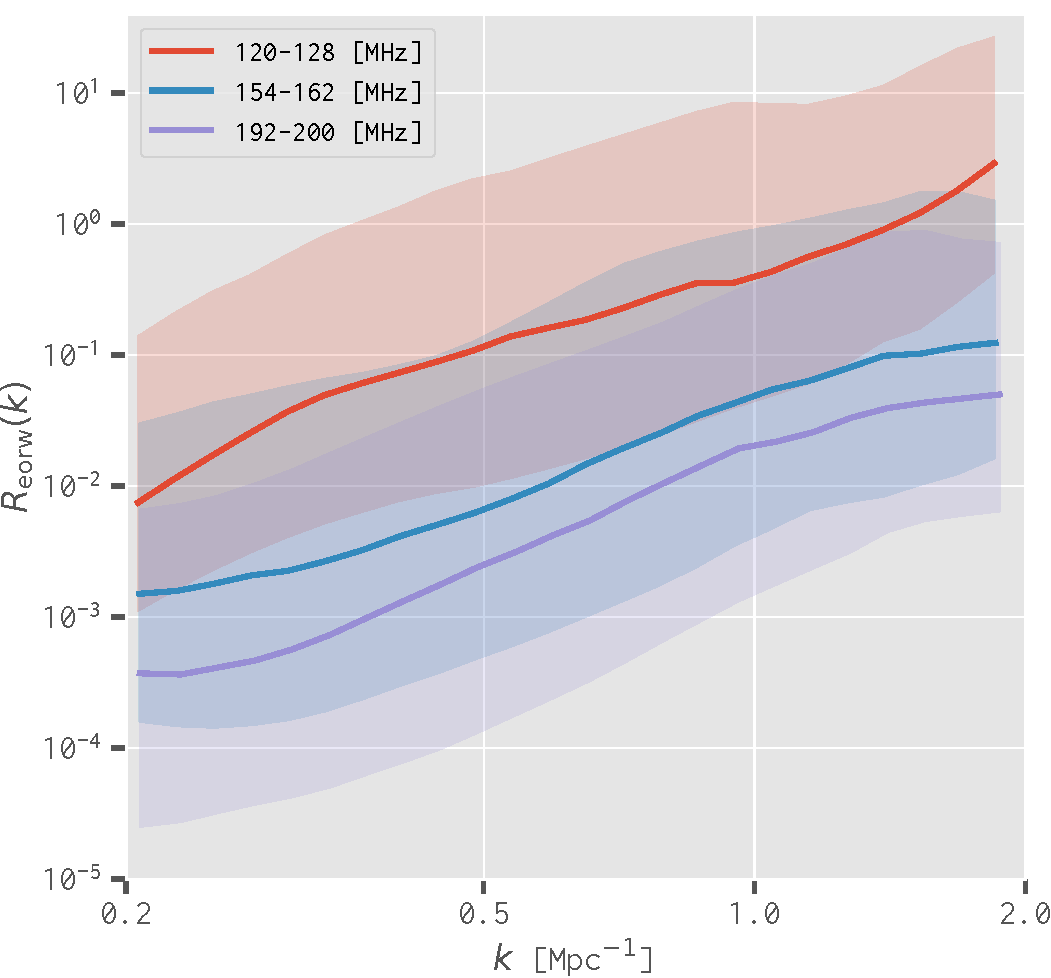
\includegraphics[width=\columnwidth]{ps1d-ratio-3bands}
      \caption{射电晕与 EoR 信号在 EoR 窗口内的一维功率比}
    \end{figure}
  \end{columns}
\end{frame}

%............
\begin{frame}{频谱伪结构的影响}
  \begin{itemize}
    \item 干涉阵列的频率通道的校准不确定性约为 0.1--1\%.
    \item 频谱伪结构幅度为 $A_{\R{arti}} = 0.1\%$ 时,
      射电晕在 $k_{\perp} \lesssim \SI{0.2}{\per\Mpc}$ 和
      $k_{\parallel} \gtrsim \SI{0.3}{\per\Mpc}$
      的功率分别增加约 17、15、13 倍.
    \item 如果 $A_{\R{arti}} = 1\%$,功率分别增加约 1700、1500、1300 倍.
  \end{itemize}

  \vspace{-1ex}
  \myfigure{%
    height=0.65\textheight,
    vertcap,
  }{ps2d-ratio-crp-3bands}{%
    有无频谱伪结构时射电晕的二维功率比
  }
\end{frame}

%............
\begin{frame}{远旁瓣的影响}
  \begin{itemize}
    \item 干涉阵列有一系列明显的旁瓣.
    \item 远离视场的源仍然可以通过旁瓣在视场中产生干扰,\\
      即\alert{远旁瓣致淆噪声 (FSCN)}.
    \item 当 $uv$ 覆盖饱和时,FSCN 便不再降低,是成像质量的限制因素之一.
  \end{itemize}

  \myfigure{%
    height=0.5\textheight,
  }{SKA1-low-beams}{%
    SKA1-Low 的站点波束
  }
\end{frame}

%............
\begin{frame}
  \begin{itemize}
    \item 模拟新的天图和观测图像:
      射电晕覆盖了从角半径 \SI{10}{\degree} 至地平线的天空范围.
    \item 射电晕 FSCN 的功率在 $k_{\perp} \sim \SI{0.3}{\per\Mpc}$ 和
      $k_{\parallel} \sim \SI{1}{\per\Mpc}$ 的功率达到了 EoR 信号的约 20 倍.
    \item 前景楔形污染向左上方大幅扩张,极大地压缩了 EoR 窗口.
  \end{itemize}

  \myfigure{%
    height=0.65\textheight,
  }{ps2d-fscn}{%
    射电晕 FSCN 的二维功率谱及其与 EoR 信号的功率谱对比
  }
\end{frame}

%............
\begin{frame}{小结}
  \begin{itemize}
    \item 射电晕是一个重要的前景干扰成分.
    \item 即使在 EoR 窗口内,射电晕的污染仍然不可忽略,尤其是在较低频率.
    \item 干涉阵列的频谱伪结构和旁瓣进一步增强了射电晕对 EoR 信号的污染.
  \end{itemize}
\end{frame}


%=====================================================================
\section{基于深度学习的 EoR 信号分离新算法}

%............
\begin{frame}{波束的频率依赖效应}
  \begin{columns}
    \column{0.5\textwidth}
    \begin{itemize}
      \item 干涉阵列的波束包含一系列旁瓣,旁瓣的位置随频率的增大而向中间移动.
      \item 干扰源所产生的辐射的位置也随频率变化.
      \item 考虑视场中某个位置,则干扰源的辐射沿频率维度出现小尺度涨落.
      \item 前景辐射的频谱光滑性受损,导致传统前景扣除方法无法有效地分离 EoR 信号.
    \end{itemize}

    \column{0.5\textwidth}
    \myfigure{%
      width=\columnwidth,
    }{cdae-simdata-example}{%
      前景辐射和 EoR 信号的频谱示例
    }
  \end{columns}
\end{frame}

%............
\begin{frame}{基于深度学习的新算法}
  \begin{itemize}
    \item 对波束效应进行手工建模几乎不可行.
    \item 研发基于\alert{深度学习}的新算法更具有可行性和吸引力:
      \begin{itemize}
        \item 自适应地从数据中汲取信息用来优化自身模型;
        \item 一旦训练好,使用过程非常高效;
        \item 灵活性高,重新训练后可应用于其他望远镜.
      \end{itemize}
  \end{itemize}
\end{frame}

%............
\begin{frame}{自编码器}
  \begin{itemize}
    \item 由\alert{编码器}和\alert{解码器}两部分组成:
      \begin{itemize}
        \item 编码器: 将输入 $\B{x}$ 映射成一个内部编码 $\B{h} = f(\B{x})$;
        \item 解码器: 尝试从编码 $\B{h}$ 重构原输入信号,$\B{r} = g(\B{h})$.
      \end{itemize}
    \item 对编码 $\B{h}$ 施加约束,训练使得重构信号 $\B{r}$ 的损失
      $L(\B{r}, \B{x})$ 最小.
    \item 学得的编码能够有效地表示输入信号.
    \item 常用于数据的降维和去噪.
  \end{itemize}

  \myfigure{width=\textwidth}{autoencoder}{自编码器的示意图}
\end{frame}

%............
\begin{frame}{去噪自编码器}
  \begin{itemize}
    \item 基于\alert{去噪准则}的全新训练策略 \cite{vincent2008,vincent2010}:
      \begin{enumerate}
        \item 人为地损坏原始输入信号 $\B{x}$,比如加入噪声;
        \item 输入受损信号 $\B{x}'$ 进行训练;
        \item 使重构信号 $\B{r}$ 尽可能地恢复原始输入信号 $\B{x}$.
      \end{enumerate}
    \item 被迫去发掘原始输入信号 $\B{x}$ 中的关键特征.
    \item 学得一个更好的表示,提升性能.
    \item 如此训练的自编码器被称为\alert{去噪自编码器}.
  \end{itemize}
\end{frame}

%............
\begin{frame}{卷积去噪自编码器 (CDAE)}
  \begin{itemize}
    \item 经典的自编码器使用\alert{全连接层}.
      主要劣势:
      \begin{itemize}
        \item 参数多,训练困难,不利于构建很深的网络;
        \item 特征是全局的,不利于描述局部特征.
      \end{itemize}
    \item 卷积神经网络 (CNN) 采用的\alert{卷积层}具有明显优势:
      \begin{itemize}
        \item 利用一组小尺寸过滤器,适合提取局部特征;
        \item 参数数目少,容易训练;
        \item 易于叠加多个卷积层,提升特征提取能力.
      \end{itemize}
    \item \alert{卷积去噪自编码器 (CDAE)}:
      \begin{itemize}
        \item 使用卷积层的去噪自编码器;
        \item 拥有更强的特征提取能力,提升去噪能力.
      \end{itemize}
  \end{itemize}

  \vspace{-1ex}
  \myfigure{width=0.85\textwidth,vertcap}{cnn}{CNN 示意图}
\end{frame}

%............
\begin{frame}{网络架构}
  \begin{itemize}
    \item 编码器: 4 层,分别包含 32、64、64、32 个过滤器;
    \item 解码器: 5 层,分别包含 32、64、64、32、1 个过滤器;
    \item 过滤器的尺寸为 3;
    \item 输出层的激活函数为 \enquote{tanh};
    \item 其余层使用\enquote{指数线性单元},
      还使用\enquote{批标准化} (BN) 技术.
  \end{itemize}
  %
  \myfigure{width=\textwidth}{cdae-network-crop}{CDAE 网络架构示意图}
\end{frame}

%............
\begin{frame}{训练和评估方法}
  \begin{itemize}
    \item 三个数据集:
      \begin{itemize}
        \item \alert{训练集 $S_{\R{tr}}$}: 拟合待训练参数;
        \item \alert{验证集 $S_{\R{val}}$}:
          验证训练过程是否正常;约束 CDAE 的超参数;
        \item \alert{测试集 $S_{\R{test}}$}:
          仅在训练结束后用于评估 CDAE 的性能.
      \end{itemize}
    \item 损失 $L(\B{r}, \B{x})$ 由\alert{均方误差}量化:
      \begin{equation}
        L = \frac{1}{N_{\R{tr}}} \sum_{i=1}^{N_{\R{tr}}}
            \left[ \B{r}_{\R{eor}}^{(i)} - \B{x}_{\R{eor}}^{(i)} \right]^T
            \left[ \B{r}_{\R{eor}}^{(i)} - \B{x}_{\R{eor}}^{(i)} \right] .
      \end{equation}
    \item 评估指标采用\alert{相关系数}:
      \begin{equation}
        \xi(\B{r}_{\R{eor}}, \B{x}_{\R{eor}})
          = \frac{\sum_{j=1}^{n}(r_{\R{eor},j} - \bar{r}_{\R{eor}})
              (x_{\R{eor},j} - \bar{x}_{\R{eor}})}{
                \sqrt{\sum_{j=1}^{n}(r_{\R{eor},j} - \bar{r}_{\R{eor}})^2
                \sum_{j=1}^{n}(x_{\R{eor},j} - \bar{x}_{\R{eor}})^2}
            } .
      \end{equation}
  \end{itemize}
\end{frame}

%............
\begin{frame}{训练数据}
  \begin{itemize}
    \item 模拟两组\enquote{观测}图像立方:
      EoR 信号 $C_{\R{eor}}$ 和前景辐射 $C_{\R{fg}}$.
      \begin{itemize}
        \item \SIrange{154}{162}{\MHz} 频带,频率分辨率 \SI{160}{\kHz},
          尺寸 \num{360 x 360};
        \item 形成数据集 $S = \left\{ \left(\B{x}^{(i)},
          \,\B{x}^{(i)}_{\R{eor}} \right) \right\}$,
          其中 $\B{x}^{(i)} = \B{x}^{(i)}_{\R{eor}} + \B{x}^{(i)}_{\R{fg}}$.
      \end{itemize}
    \item 预处理输入数据 $X = \big\{ \B{x}^{(i)} \big\}$
      和输入 EoR 信号 $X_{\R{eor}} = \big\{ \B{x}^{(i)}_{\R{eor}} \big\}$.
    \item 划分为三个数据集:
      \begin{itemize}
        \item $\left( C_{\R{eor}}^{(1)}, C_{\R{fg}}^{(1)} \right)$
          按 80\% 和 20\% 划分为训练集 $S_{\R{tr}}$ 和验证集 $S_{\R{val}}$;
        \item $\left( C_{\R{eor}}^{(2)}, C_{\R{fg}}^{(2)} \right)$
          全部用于测试集 $S_{\R{test}}$.
      \end{itemize}
  \end{itemize}
\end{frame}

%............
\begin{frame}{训练结果}
  \begin{itemize}
    \item 损失 $L_{\R{tr}}$ 和 $L_{\R{val}}$ 持续减小,
      相关系数 $\xi_{\R{val}}$ 稳步增长;
    \item 训练效果很好,无过拟合;
    \item 利用测试集 $S_{\R{test}}$,
      平均相关系数达 $\bar{\xi} = \num{0.929 +- 0.045}$.
  \end{itemize}

  \vspace{-1ex}
  \myfigure{%
    width=0.8\textwidth,
  }{cdae-train}{CDAE 的训练过程和结果}
\end{frame}

%............
\begin{frame}{EoR 信号分离效果}
  \vspace{-1ex}
  \myfigure{%
    height=0.9\textheight,
  }{cdae-eor-pix}{CDAE 重构的 EoR 信号的示例 ($\xi = 0.931$)}
\end{frame}

\begin{frame}
  \vspace{1ex}
  \begin{itemize}
    \item 重构的 EoR 图像的空间结构与强度分布与输入几乎完全相同;
    \item 小尺度波纹结构源自预处理时去除了低频 Fourier 系数.
      \par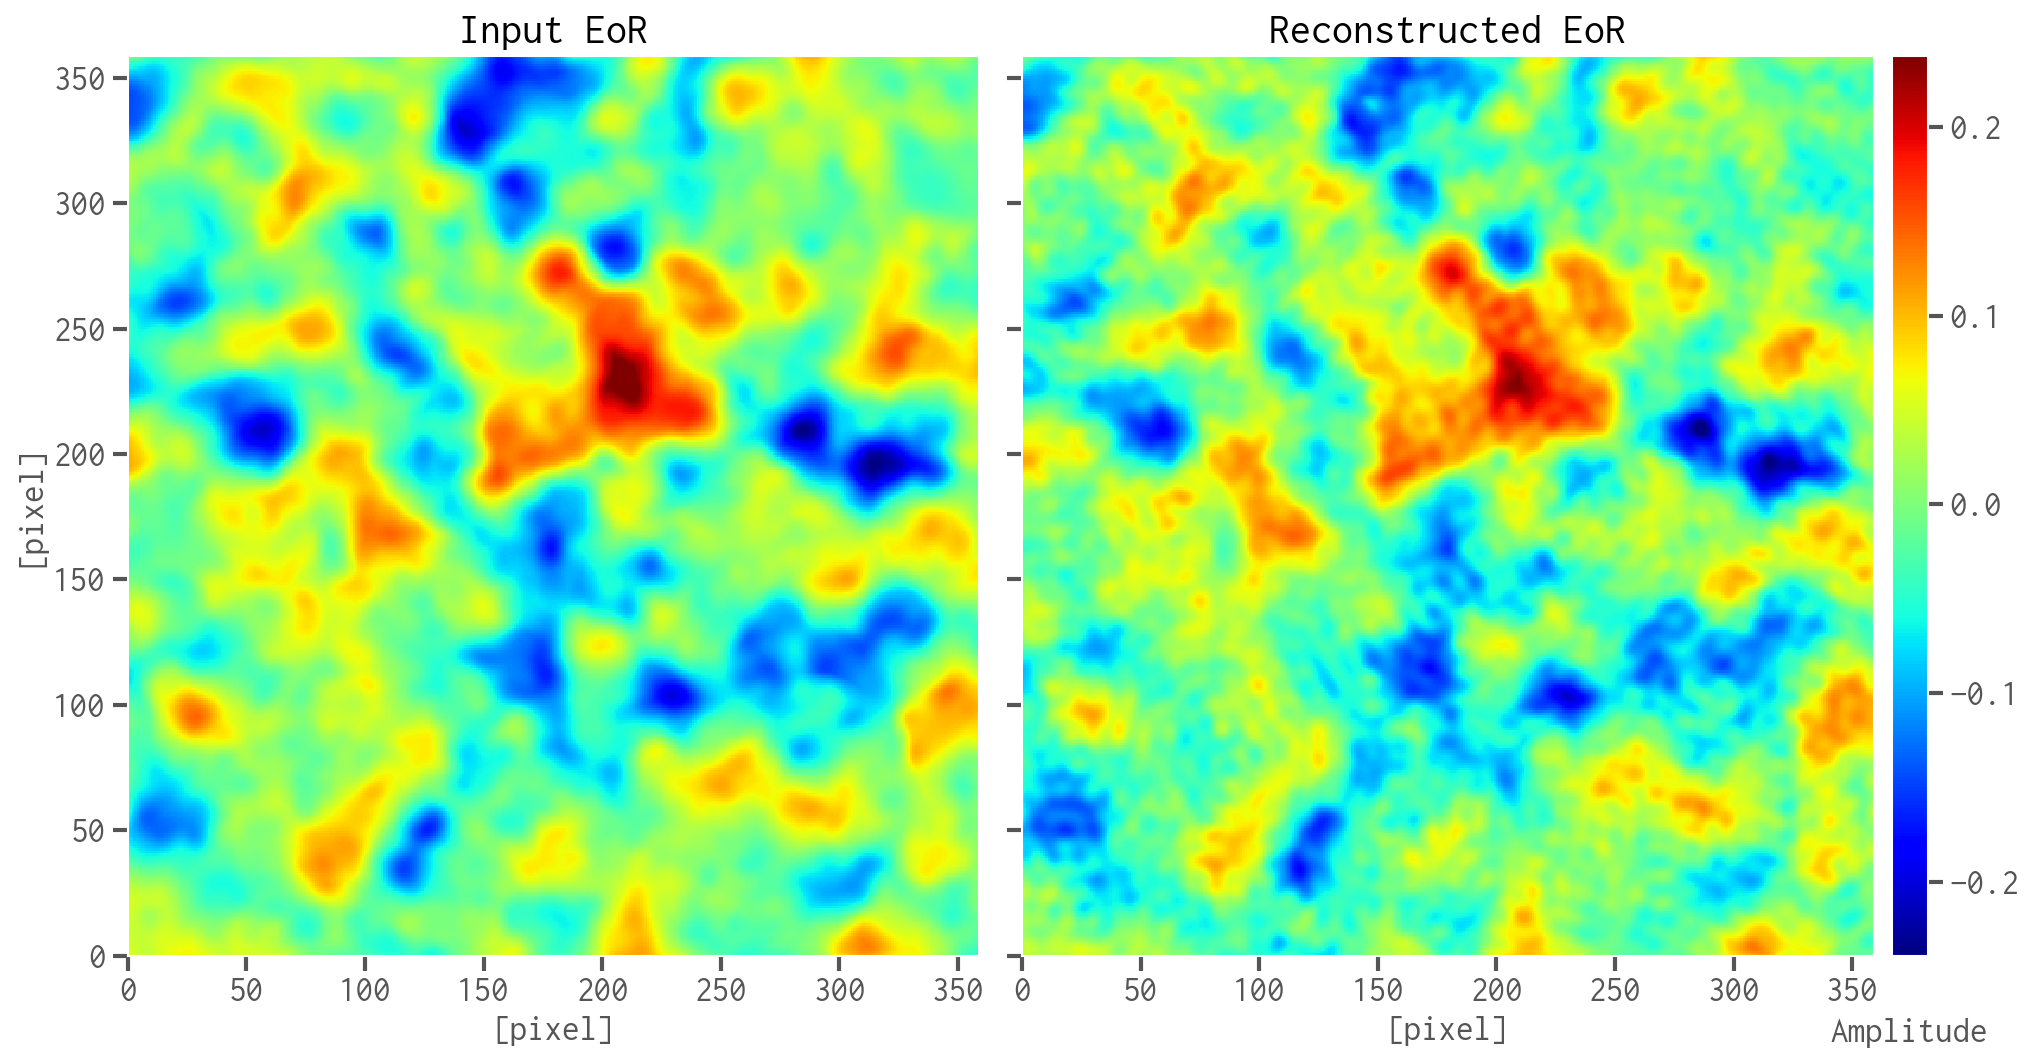
\includegraphics[height=0.44\textheight]{cdae-eor-img-comp}
    \item CDAE 很好地恢复了 EoR 信号在各尺度的功率.
      \par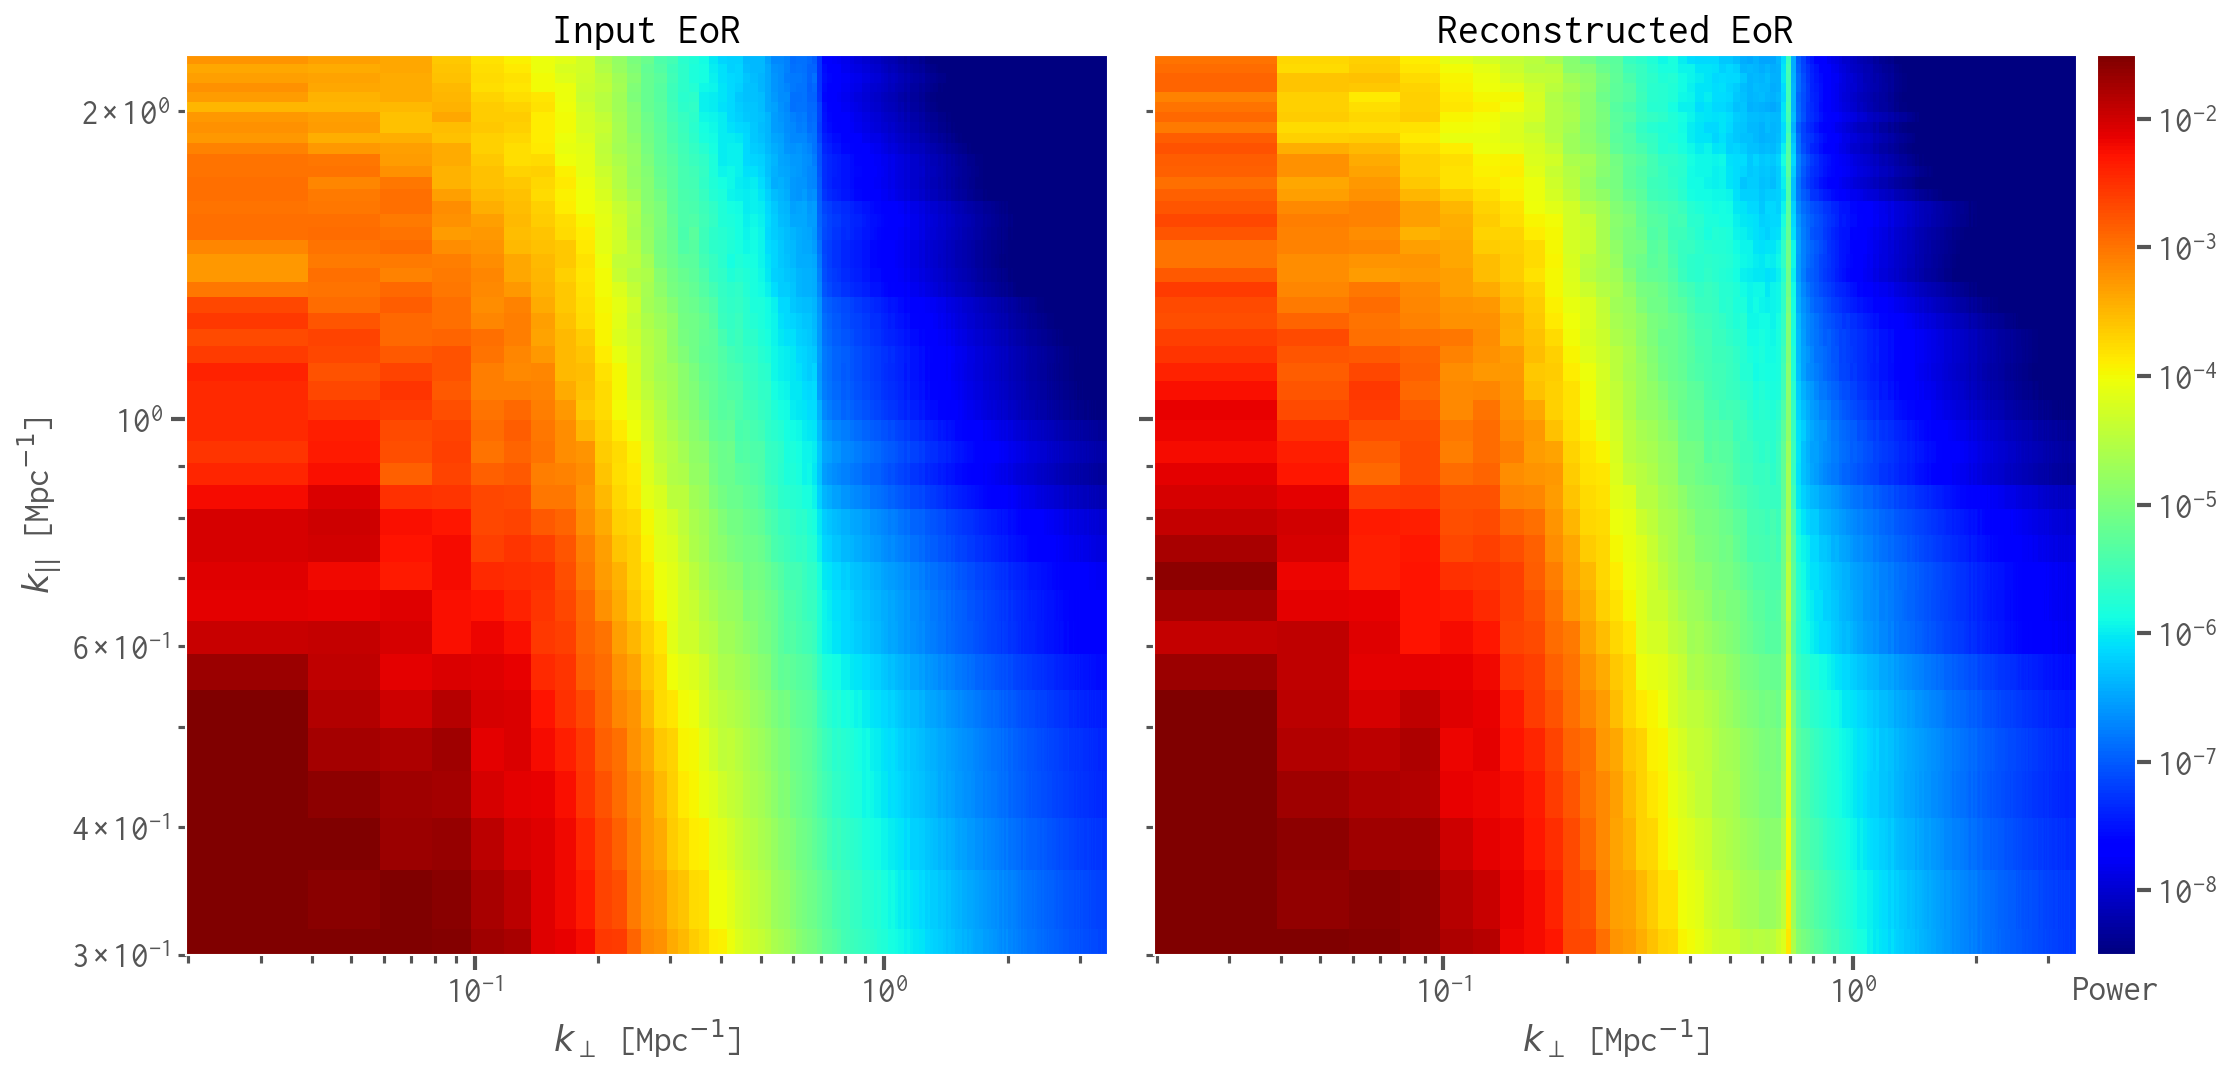
\includegraphics[height=0.44\textheight]{cdae-eor-ps-comp}
  \end{itemize}
\end{frame}

%............
\begin{frame}{与传统方法的对比}
  \begin{itemize}
    \item 传统的前景扣除法可分为\alert{参数化方法}和\alert{非参数化方法}.
    \item 参数化方法:
      \begin{itemize}
        \item 使用一个参数化模型来拟合前景辐射;
        \item 选取\alert{多项式拟合法}为代表;
        \item 分离效果仅有: $\bar{\xi}_{\R{poly}} = \num{0.296 +- 0.121}$.
      \end{itemize}
    \item 非参数化方法:
      \begin{itemize}
        \item 利用前景辐射与 EoR 信号的频谱结构差异,但不假定一个特定的参数化模型;
        \item 选取\alert{连续小波变换法}\cite{gu2013}为代表;
        \item 分离效果仅达到: $\bar{\xi}_{\R{cwt}} = \num{0.198 +- 0.160}$.
      \end{itemize}
    \item 两种传统方法均难以对复杂的前景辐射建模并扣除.
  \end{itemize}
\end{frame}

%............
\begin{frame}{小结}
  \begin{itemize}
    \item 波束效应会破坏前景频谱的光滑性,导致传统的前景扣除方法失效.
    \item 基于深度学习方法设计了一个由 9 个卷积层构成的 CDAE,
      经过训练后能够准确地分离 EoR 信号,效果显著优于传统方法.
  \end{itemize}
\end{frame}


%=====================================================================
\section{总结}

\begin{frame}{总\cspace{}结}
  \begin{itemize}
    \item 借助 PS 理论和湍流再加速模型,对射电晕的形成和演化过程进行了完整的建模,
      显著改进了射电晕的低频射电天图的模拟.
    \item 采用目前最新的 SKA1-Low~阵列布局,对模拟天图展开模拟观测,
      将干涉阵列的复杂仪器效应整合到模拟图像之中.
    \item 利用一维和二维功率谱,充分评估了射电晕对 EoR 探测的干扰行为,
      说明射电晕是一个重要的前景干扰成分.
    \item 基于深度学习方法,设计了一个卷积去噪自编码器,
      准确地分离出 EoR 信号,成功克服了复杂的波束效应.
  \end{itemize}
\end{frame}

\begin{frame}{已发表论文}
  \small
  \begin{itemize}
    \item
      \textsc{\alert{Li, Weitian}; Xu, Haiguang; Ma, Zhixian; Hu, Dan;
      Zhu, Zhenghao; Shan, Chenxi; Wang, Jingying; Gu, Junhua;
      Zheng, Dongchao; Lian, Xiaoli; Zheng, Qian; Wang, Yu;
      Zhu, Jie; Wu, Xiang-Ping}.
      \enquote{\it Contribution of Radio Halos to the Foreground for
        SKA EoR Experiments,}
      \href{http://adsabs.harvard.edu/abs/arXiv:1905.05399}{%
        2019, ApJ, accepted}
    \item
      \textsc{\alert{Li, Weitian}; Xu, Haiguang; Ma, Zhixian; Zhu, Ruimin;
      Hu, Dan; Zhu, Zhenghao; Gu, Junhua; Shan, Chenxi; Zhu, Jie;
      Wu, Xiang-Ping}.
      \enquote{\it Separating the EoR Signal with a Convolutional Denoising
        Autoencoder: A Deep-learning-based Method,}
      \href{http://adsabs.harvard.edu/abs/2019MNRAS.485.2628L}{%
        2019, MNRAS, 485, 2628}
    \item
      合作论文 12 篇
  \end{itemize}
\end{frame}

\begin{frame}[standout]
  \Huge 谢\cspace{}谢

  \note[item]{感谢导师}
  \note[item]{感谢评审专家}
\end{frame}


%=====================================================================
\appendix

\begin{frame}[standout]
  Backup slides
\end{frame}

%............
\begin{frame}{辐射转移}
  \begin{itemize}
    \item 辐射在介质中传播时会经历吸收和发射,由\alert{辐射转移方程}描述:
      \begin{equation}
        \diff{I_{\nu}}{s} = -\kappa I_{\nu} + j_{\nu} ,
      \end{equation}
      其中 $\kappa$ 为吸收系数, $j_{\nu}$ 为发射系数.
    \item \alert{光深}:
      \begin{equation}
        \tau \equiv
          - \int_{s_{\R{out}}}^{s_{\R{in}}} \kappa(s') \,\D{s'} .
      \end{equation}
      当 $\tau \ll 1$ 时,称介质是\emph{光学薄}的;
      当 $\tau \gg 1$ 时,则称介质是\emph{光学厚}的.
  \end{itemize}
\end{frame}

%............
\begin{frame}{干涉测量原理}
  \begin{columns}
    \column{0.4\textwidth}
    二元准单色干涉仪观测一个点源,相关器的输出响应为:
    \begin{align}
      R & = \langle V_1(t) V_2(t) \rangle \\
        & = \frac{1}{2} V^2 \cos (\omega \tau_g) ,
    \end{align}
    $\tau_g = \B{b} \cdot \hat{\B{s}}$ 为几何延迟,\\
    $\B{b}$ 为基线矢量,\\
    $\hat{\B{s}}$ 为辐射源的方向.

    \column{0.6\textwidth}
    \begin{figure}
      \centering
      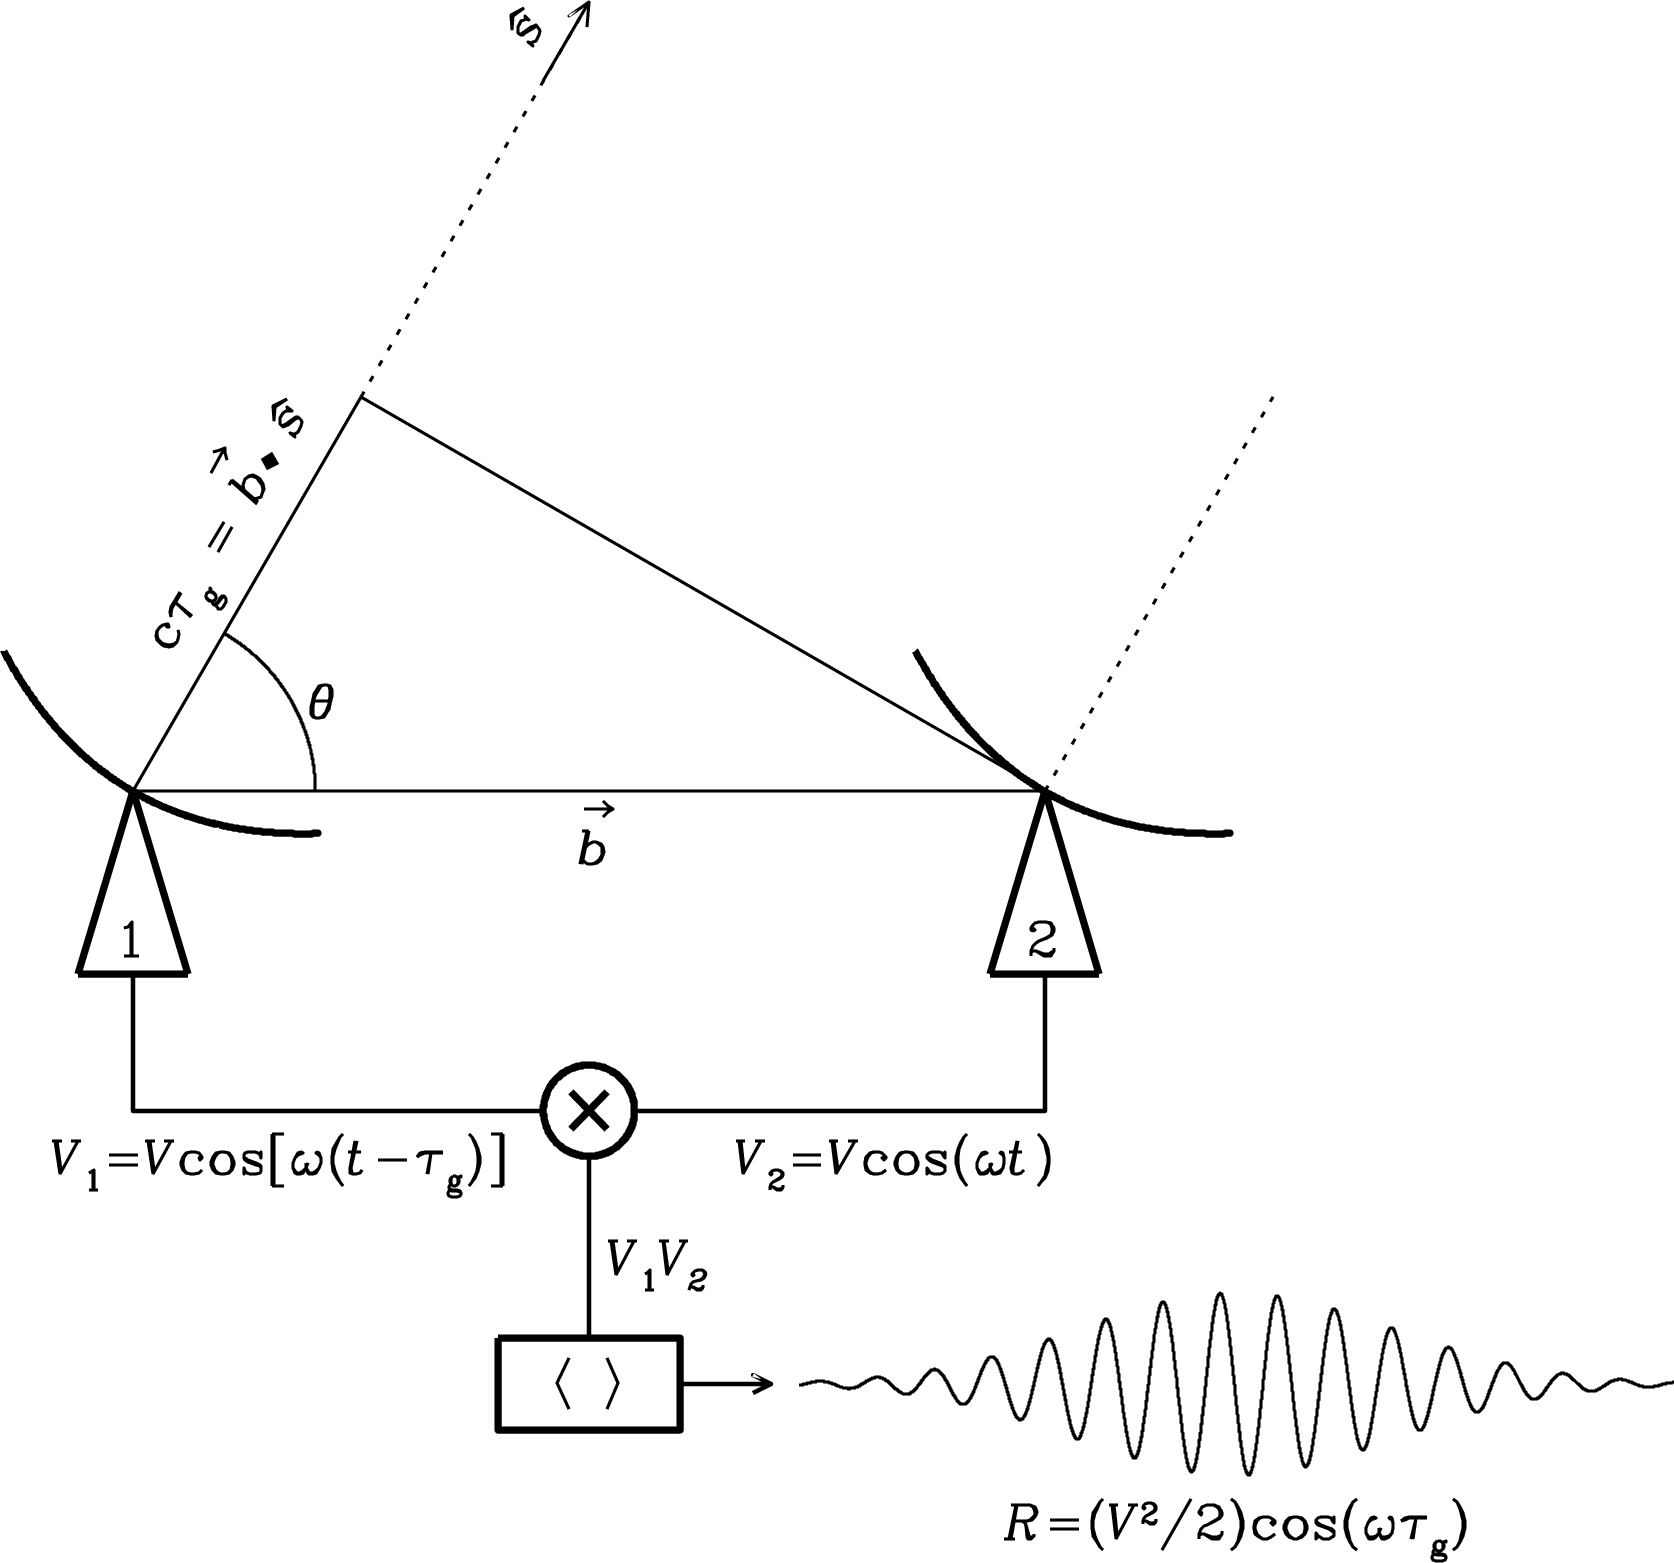
\includegraphics[width=\columnwidth]{interferometer}
      \caption{二元准单色干涉仪示意图 (\citeay{condon2016})}
    \end{figure}
  \end{columns}
\end{frame}

%............
\begin{frame}
  \begin{itemize}
    \item 一个展源 $I_{\nu}(\hat{\B{s}})$ 可当作一系列独立的点源处理,
      于是干涉仪响应为:
      \begin{equation}
        R_c = \int I_{\nu}(\hat{\B{s}})
          \cos (2\Cpi\, \B{b} \cdot \hat{\B{s}} / \lambda) \,\D{\Omega} .
      \end{equation}
    \item 上述 \enquote{cosine} 相关器只能测量 $I_{\nu}(\hat{\B{s}})$ 的偶成分.
    \item 为测量 $I_{\nu}(\hat{\B{s}})$ 的奇成分,
      还需要一个 \enquote{sine} 相关器,
      可通过对其中一个天线的输出增加 $\Cpi/2$ 的相位延迟来实现,于是:
      \begin{equation}
        R_s = \int I_{\nu}(\hat{\B{s}})
          \sin (2\Cpi\, \B{b} \cdot \hat{\B{s}} / \lambda) \,\D{\Omega} .
      \end{equation}
    \item \alert{复可见度 (complex visibility)} 定义为:
      \begin{equation}
        \mathcal{V}
          \equiv R_c - \Ci R_s
          = \int I_{\nu}(\hat{\B{s}})
            \exp (- 2\Cpi\Ci\, \B{b} \cdot \hat{\B{s}} / \lambda)
            \,\D{\Omega} .
      \end{equation}
  \end{itemize}
\end{frame}

%............
\begin{frame}{坐标系统}
  \begin{columns}
    \column{0.55\textwidth}
    \begin{itemize}
      \item $w$ 轴指向参考方向,通常为目标的中心; \\
        $u$ 轴向东; \\
        $v$ 轴向北.
      \item 基线矢量: $\B{b} = (u,v,w) \,\lambda$.
      \item 方向矢量: $\hat{\B{s}} = \left( l, m, \sqrt{1-l^2-m^2} \right)$,
        其中 $l, m$ 分别为 $\hat{\B{s}}$ 对 $u, v$ 轴的投影长度.
    \end{itemize}

    \column{0.4\textwidth}
    \begin{figure}
      \centering
      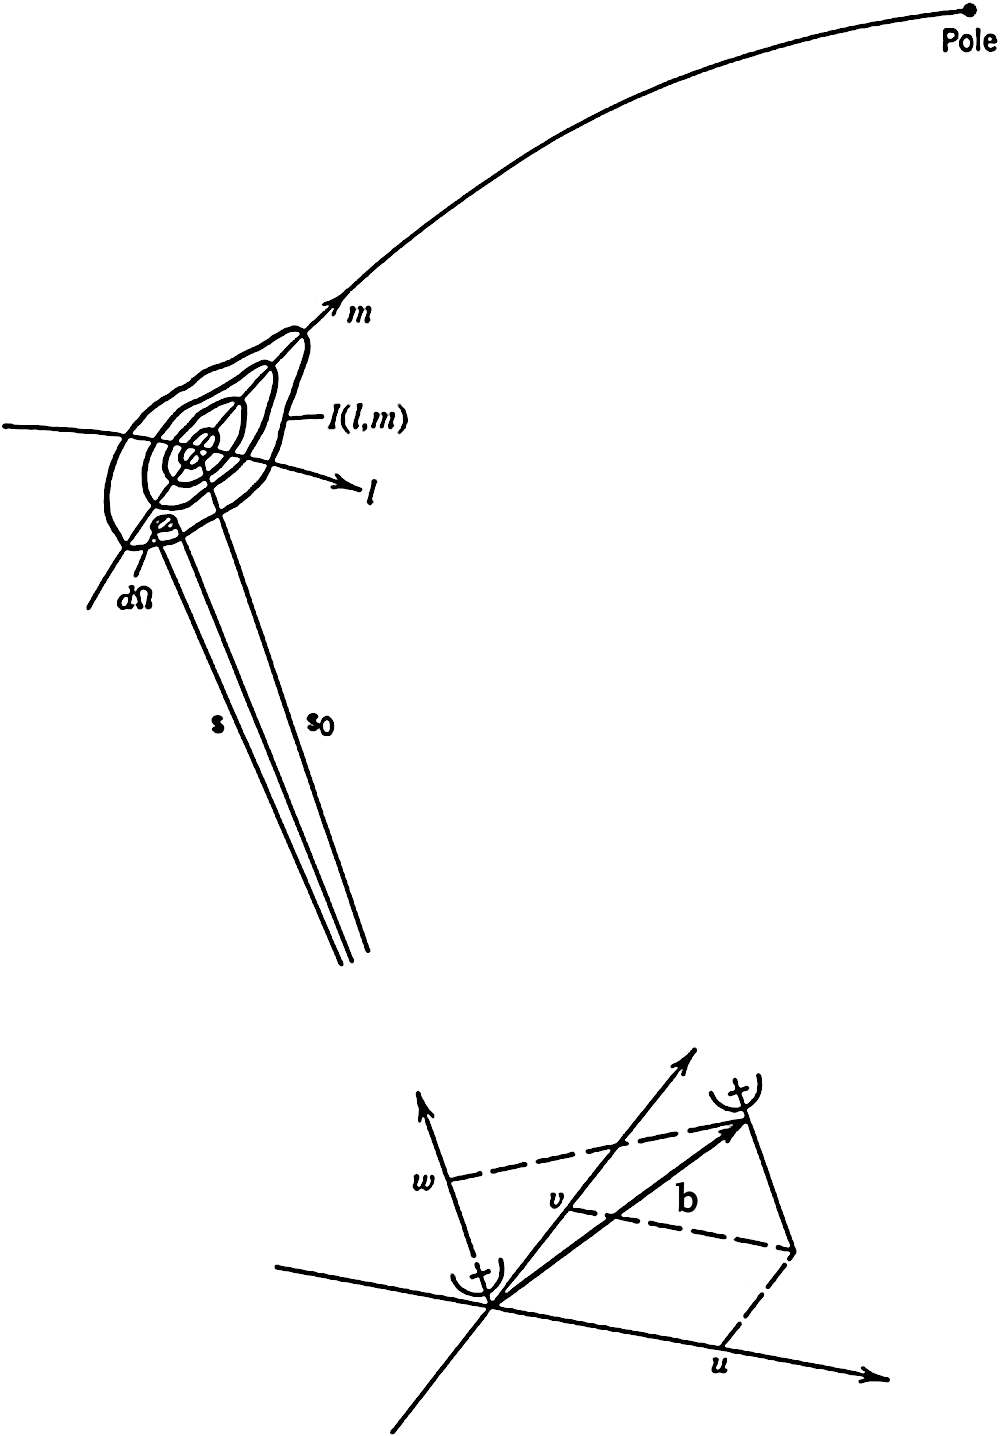
\includegraphics[width=\columnwidth]{interferometer-coordsys}
      \caption{干涉仪的 $(u,v,w)$ 直角坐标系 (\citeay{thompson2017})}
    \end{figure}
  \end{columns}
\end{frame}

%............
\begin{frame}{成像原理}
  \begin{equation}
    \mathcal{V}(u,v,w)
      = \!\iint \!\frac{I_{\nu}(l,m)}{\sqrt{1-l^2-m^2}}
      \exp \!\left[ -2\Cpi\Ci \!\left( ul+vm+w\sqrt{1-l^2-m^2} \right) \right]
      \D{l}\,\D{m}
  \end{equation}

  \begin{itemize}
    \item 注意,上式\alert{不是}二维 Fourier 变换.
    \item 在以下两种常见的特殊情况下:
      \begin{itemize}
        \item 所有基线矢量共面,即有 $w = 0$;
        \item 小视场成像,即满足 $\big| \Cpi w(l^2+m^2) \big| \ll 1$.
      \end{itemize}
      上式可近似成二维 Fourier 变换:
      \begin{equation}
        \mathcal{V}(u,v)
          = \iint \frac{I_{\nu}(l,m)}{\sqrt{1-l^2-m^2}}
            \exp [-2\Cpi\Ci\, (ul+vm)] \,\D{l}\,\D{m},
      \end{equation}
    \item 通过逆变换,可得目标的亮度分布 $I_{\nu}(l,m)$:
      \begin{equation}
        \frac{I_{\nu}(l,m)}{\sqrt{1-l^2-m^2}}
          = \iint \mathcal{V}(u,v)
            \exp [2\Cpi\Ci\, (ul+vm)] \,\D{l}\,\D{m}.
      \end{equation}
  \end{itemize}
\end{frame}

%............
\begin{frame}{$uv$ 覆盖}
  \begin{itemize}
    \item 基线 $\B{b} = (u,v,w) \,\lambda$ 每个时刻测量一对可见度数据: \\
      $\mathcal{V}(u,v)$ 和 $\mathcal{V}(-u,-v)$.
    \item \alert{$uv$ 覆盖}指 $uv$ 平面内被测量到的范围,
      由\alert{采样函数} $S(u,v)$ 描述.
    \item 对测量的可见度数据进行逆 Fourier 变换,
      仅能得到目标的\alert{脏图 (dirty map)}:
      \begin{equation}
        \frac{I_{\nu}^D(l,m)}{\sqrt{1-l^2-m^2}}
          = \iint \mathcal{V}(u,v) S(u,v)
            \exp [2\Cpi\Ci\, (ul+vm)] \,\D{l}\,\D{m}.
      \end{equation}
    \item \alert{综合波束 (synthesized beam)}
      或\alert{点扩散函数 (point spread function; PSF)}
      是 $S(u,v)$ 的 Fourier 变换:
      \begin{equation}
        B(l,m) = \iint S(u,v) \exp [2\Cpi\Ci\, (ul+vm)] \,\D{l}\,\D{m}.
      \end{equation}
  \end{itemize}
\end{frame}

%............
\begin{frame}{成像过程的变换关系}
  \begin{figure}
    \centering
    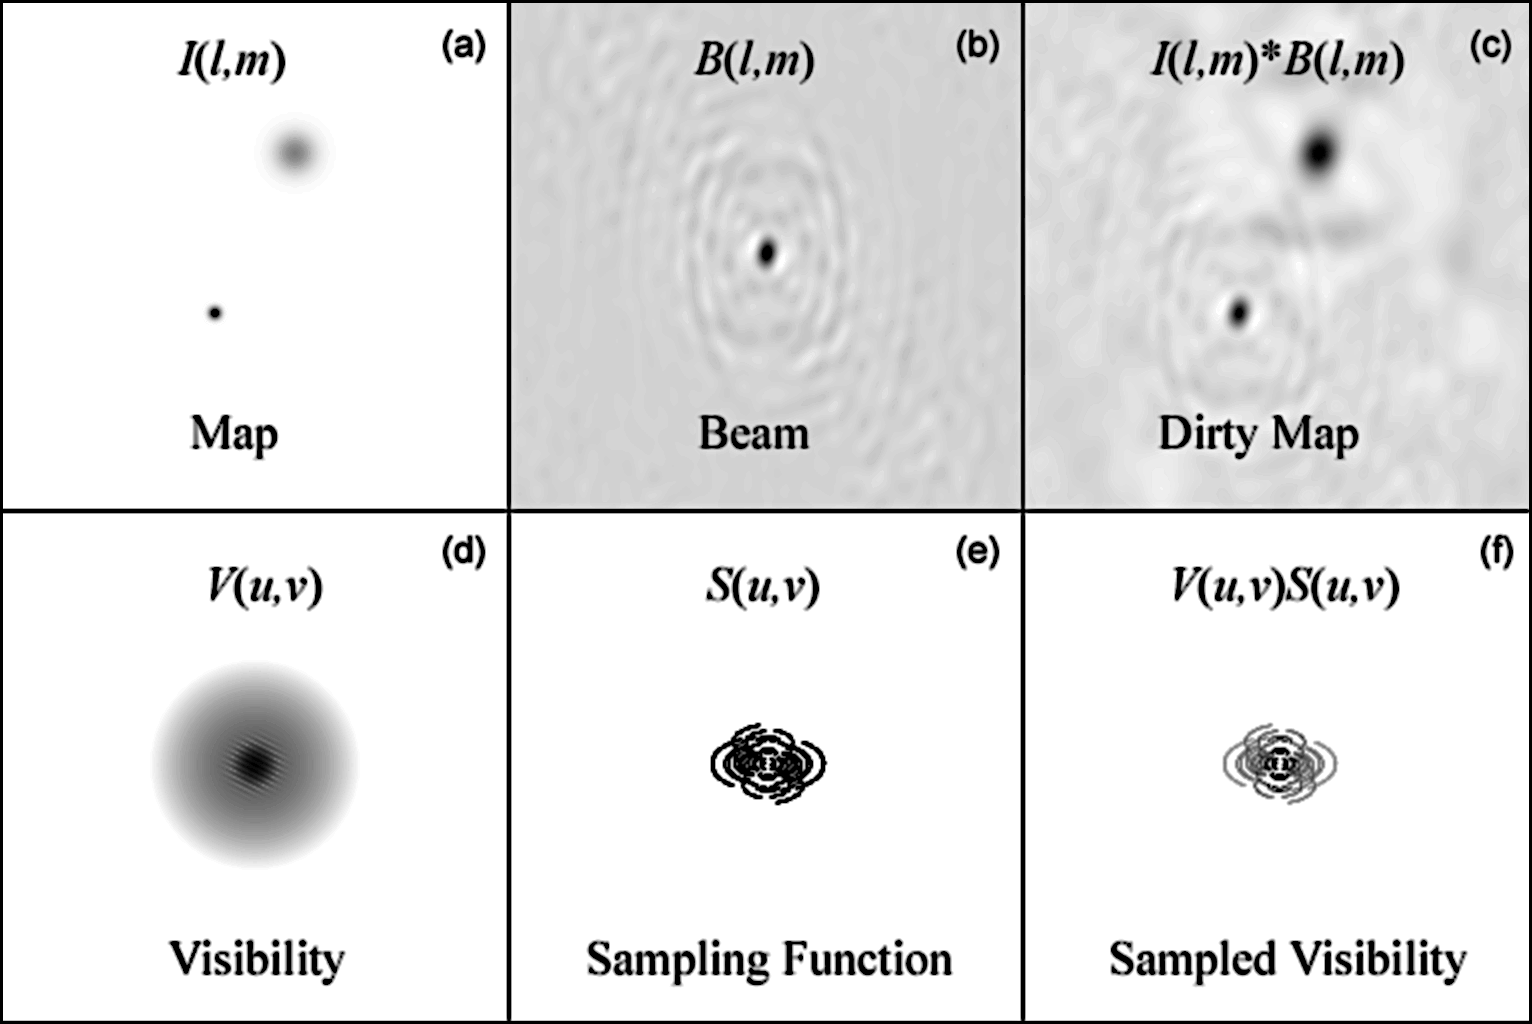
\includegraphics[width=0.9\textwidth]{imaging-relations}
    \caption{%
      (a) 真实图像;
      (b) 综合波束;
      (c) 脏图;
      (d) 真实的可见度数据;
      (e) 采样函数;
      (f) 测量到的可见度数据.
      (Dale E. Gary, Radio Astronomy)
    }
  \end{figure}
\end{frame}

\begin{frame}[allowframebreaks]{参考文献}
  \printbibliography[heading=none]
\end{frame}

\end{document}
